\documentclass{beamer}

\usetheme{Madrid} % A clean, popular theme
\usecolortheme{default}
\usefonttheme{professionalfonts}

\usepackage[utf8]{inputenc}
\usepackage[T1]{fontenc}
\usepackage{amsmath}
\usepackage{amssymb}
\usepackage{graphicx}
\usepackage{booktabs} % For nice tables
\usepackage{subcaption} % For subfigures
\usepackage{hyperref}
\usepackage{xcolor}
\usepackage{enumerate} % For custom enumerate labels
\usepackage{array} % For advanced column types

\usepackage[style=authoryear]{biblatex}
\addbibresource{report.bib}

% Define a title page
\title{Sovereign Debt Relief and Its Aftermath \\ Replication Report Presentation}
\subtitle{Carmen M. Reinhart, Christoph Trebesch}
\author{Jingle Fu / Yingjie Zhang / Zhixu Liu}
\date{\today}

% For section/subsection pages
\AtBeginSection[]
{
  \begin{frame}
    \vfill
    \centering
    \begin{beamercolorbox}[sep=8pt,center,shadow=true,rounded=true]{title}
      \usebeamerfont{title}\insertsectionhead\par
    \end{beamercolorbox}
    \vfill
  \end{frame}
}

% \AtBeginSubsection[]
% {
%   \begin{frame}
%     \vfill
%     \centering
%     \begin{beamercolorbox}[sep=8pt,center,shadow=true,rounded=true]{title}
%       \usebeamerfont{subtitle}\insertsectionhead\par
%       \bigskip
%       \usebeamerfont{frametitle}\insertsubsectionhead\par
%     \end{beamercolorbox}
%     \vfill
%   \end{frame}
% }


\begin{document}

\begin{frame}
  \titlepage
\end{frame}

\begin{frame}{Outline}
  \tableofcontents
\end{frame}

\section{Introduction}

\subsection{Key Question and Contribution}
\begin{frame}{Key Question}
  \begin{block}{Key Question}
    Should countries with a heavy debt burden and little prospect of repayment receive debt forgiveness?
  \end{block}
  \begin{itemize}
    \item Literature has mostly focused on the \textit{occurrence} of debt crises, not on their \textit{resolution}.
    \item \textbf{Contribution of this paper:} Filling this gap by studying two 20th century instances of debt relief encompassing a substantial number of countries.
  \end{itemize}
\end{frame}

\subsection{Key Challenges and Solutions}
\begin{frame}{Key Challenges and Methodological Solutions}
  \begin{enumerate}
    \item \textbf{Timing of debt relief may be endogenous.}
    \begin{itemize}
        \item \textit{Solution:} Focus on episodes of debt reduction synchronously applied across debtor countries, regardless of individual economic circumstances.
        \item Examples:
        \begin{itemize}
            \item 1931 Hoover Moratorium (cash flow relief)
            \item 1934 General Default on War Debts (debt stock relief)
            \item 1986 Baker Plan (reducing interest rates, lengthening maturities)
            \item 1990 Brady Initiative (face value debt reduction)
        \end{itemize}
    \end{itemize}
    \item \textbf{Omitted variables and other factors.}
    \begin{itemize}
        \item \textit{Solution:}
        \begin{itemize}
            \item Add time and country fixed effects (core to DiD).
            \item Robustness checks: adding controls for inflation, banking/currency crises, wars, political shocks.
        \end{itemize}
    \end{itemize}
  \end{enumerate}
\end{frame}

% --- CHAPTER 2: Basic Facts ---
\section{Basic Facts}

\subsection{The 1934 General Default on War Debts}
\begin{frame}{The 1934 General Default on War Debts}
  \label{sec:1934generaldefault}
  \begin{itemize}
    \item In 1934, all European countries (except Finland) stopped paying their war debts to the US and UK.
    \item The US, despite strong opposition, could not enforce repayment.
    \item This event is characterized as a form of `debt relief'.
    \item The US Treasury still lists these unpaid 1934 war debt obligations.
    \item \textbf{Notable Exception}: Finland was the only country that paid off its war debts.
  \end{itemize}
\end{frame}

\subsection{Data Resources}
\begin{frame}{Data Resources}
  \begin{itemize}
    \item \textbf{Primary Sources}:
    \begin{itemize}
        \item United Nations 1948 publication: \textit{Public Debt, 1914-1946}.
        \item Annual financial reports by the US Treasury Department.
    \end{itemize}
    \item \textbf{Data Consistency}:
    \begin{itemize}
        \item Numbers across sources are generally similar, with slight differences.
        \item Authors attribute differences to exchange rates or other factors.
    \end{itemize}
    \item \textbf{Valuation of Debt Relief}:
    \begin{itemize}
        \item The exchange rate of 1934 is used to estimate the value of debt relief, as 1934 is the 'formal' year of relief.
    \end{itemize}
    \item \textbf{Estimation Approach}:
    \begin{itemize}
        \item Authors use the most conservative estimates of debt relief when best sources are unavailable.
    \end{itemize}
  \end{itemize}
\end{frame}

% % ---------- Frame 1 ----------
% \begin{frame}[fragile]{Interwar dataset: variable documentation (1/2)}
%   \scriptsize
%   \centering
%   \begin{tabular}{cc}
%   \toprule
%   \textbf{Variable} & \textbf{Description} \\
%   \midrule
%   \texttt{countrypanelid} & Internal country-year panel identifier \\
%   \texttt{country} & Country name \\
%   \texttt{year\_str} & Year (string) \\
%   \texttt{year} & Year (numeric) \\
%   \texttt{countrycodeid} & Country code identifier \\
%   \texttt{code} & ISO 3166-3 alphabetic country code \\
%   \texttt{codeid} & Same as \texttt{code}, stored as a category field \\
%   \texttt{gdp\_real\_Maddison\_TED} & Real GDP (1990 USD, PPP; Maddison/TED) \\
%   \texttt{gdp\_pc\_real\_Maddison\_TED} & Real GDP per capita (1990 USD; Maddison/TED) \\
%   \texttt{gdp\_nominal\_Maddison\_TED} & Nominal GDP (Maddison/TED) \\
%   \texttt{gdp\_pc\_nominal\_Maddison\_TED} & Nominal GDP per capita (Maddison/TED) \\
%   \texttt{gdp\_deflator} & GDP deflator (2009 = 100) \\
%   \texttt{growth\_gdp\_real\_Maddison\_TED} & Real GDP year-on-year growth (\%) \\
%   \texttt{growth\_gdp\_pc\_real\_Maddison\_TED} & Real GDP per capita YoY growth (\%) \\
%   \texttt{GDP\_devtrend\_interwar} & Deviation of log GDP from trend (HP-filter cycle) \\
%   \bottomrule
%   \end{tabular}
% \end{frame}

% % ---------- Frame 2 ----------
% \begin{frame}[fragile]{Interwar dataset: variable documentation (2/2)}
% \scriptsize
% \centering
% \begin{tabular}{cc}
% \toprule
% \textbf{Variable} & \textbf{Description} \\
% \midrule
% \texttt{debt\_gdpAbbas} & General-government gross debt / GDP (Abbas et al.) \\
% \texttt{ext\_debt\_gdp} & External debt / GDP (Reinhart & Rogoff) \\
% \texttt{debtservGDP\_interwar} & Debt service / GDP \\
% \texttt{debtservRevenue\_interwar} & Debt service / government revenue \\
% \texttt{moodys\_interwar\_num} & Moody's sovereign rating (numeric, lower = better) \\
% \texttt{Intrastateconflict} & Intrastate conflict index (Correlates of War) \\
% \texttt{InterstateConflict} & Interstate conflict index (Correlates of War) \\
% \texttt{inflation\_RR} & Inflation rate (Reinhart & Rogoff) \\
% \texttt{bankingcrises} & Banking-crisis dummy (R & R database) \\
% \texttt{currencycrises} & Currency-crisis dummy (R & R database) \\
% \texttt{domestic1} & Number of assassinations \\
% \texttt{domestic3} & Number of guerrilla-warfare events \\
% \texttt{domestic4} & Number of government-crisis events \\
% \texttt{domestic6} & Number of riots \\
% \texttt{domestic7} & Number of revolutions \\
% \bottomrule
% \end{tabular}
% \end{frame}


% % ---------- Frame 1 ----------
% \begin{frame}[fragile]{EMEs dataset: variable documentation (1/2)}
% \scriptsize
% \centering
% \begin{tabular}{cc}
% \toprule
% \textbf{Variable} & \textbf{Description} \\
% \midrule
% \texttt{countrypanelid}        & Internal country-year panel identifier \\
% \texttt{country}               & Country name \\
% \texttt{year\_str}             & Year (string) \\
% \texttt{year}                  & Year (numeric) \\
% \texttt{countrycodeid}         & Country code identifier \\
% \texttt{code}                  & ISO 3166 alpha-3 code \\
% \texttt{codeid}                & ISO 3166 alpha-3 code (categorical) \\
% \texttt{debt\_gdpAbbas}        & Debt / GDP (Abbas et al. 2011) \\
% \texttt{DebtService\_Exports}  & Debt service / exports (World Bank) \\
% \texttt{DebtExt\_GNI}          & Total external debt / GNI (World Bank) \\
% \texttt{DebtServTotal\_GDP}    & Debt service / GDP (World Bank) \\
% \texttt{EME\_real\_pc}         & Real GDP per capita \\
% \texttt{EME\_real\_pc\_growth} & Growth of real GDP per capita \\
% \texttt{Intrastateconflict}    & Internal conflict index (COW) \\
% \texttt{InterstateConflict}    & External conflict index (COW) \\
% \bottomrule
% \end{tabular}
% \end{frame}

% % ---------- Frame 2 ----------
% \begin{frame}[fragile]{EMEs dataset: variable documentation (2/2)}
% \scriptsize
% \centering
% \begin{tabular}{cc}
% \toprule
% \textbf{Variable} & \textbf{Description} \\
% \midrule
% \texttt{inflation\_RR} & Inflation rate \\
% \texttt{bankingcrises} & Banking-crisis dummy \\
% \texttt{currencycrises} & Currency-crisis dummy \\
% \texttt{domestic4} & Government-crisis events \\
% \texttt{domestic6} & Riots \\
% \texttt{domestic7} & Revolutions \\
% \texttt{iir\_yearly} & Institutional Investor rating (0-100) \\
% \bottomrule
% \end{tabular}
% \end{frame}


% --- CHAPTER 3: Key Mathematical Model ---
\section{Key Mathematical Model}

% \subsection{Haircut Calculations for Emerging Markets}
\begin{frame}{Haircut Calculations: Identification Challenge}
  \label{sec:haircutcalc}
  \begin{itemize}
    % \item \textbf{Cited Works} (among others): \cite{borusyak2021revisiting}, \cite{cruces2013sovereign}, \cite{reinhart2016sovereign}, \cite{sturzenegger2006debt}.
    \item \textbf{Main Identification Challenge}: The timing of debt relief events might be endogenous to a country's economic situation.
    \item \textbf{Authors' Approach}:
    \begin{itemize}
        \item Use four major debt relief events as quasi-natural experiments.
        \item These events were coordinated by governments and involved multiple debtor countries.
        \item Argued to be principally exogenous to the economic situation of individual countries.
        \item Events not related to specific debt negotiations that could be endogenous.
        \item Example: Hoover Moratorium (1931) began after 15 countries had already defaulted for 2 years; all 18 countries defaulted by 1934 (Cruces and Trebesch, 2013, Appendix B).
    \end{itemize}
  \end{itemize}
\end{frame}

% \subsection{Heterogeneous Haircuts}
\begin{frame}{Heterogeneous Haircuts}
  \begin{itemize}
    \item \textbf{Debt Flow Relief (Rescheduling \& Delayed Repayments)}:
    \begin{itemize}
        \item Hoover operations
        \item Baker operations
    \end{itemize}
    \item \textbf{Debt Stock Relief (Reduced Nominal Value)}:
    \begin{itemize}
        \item 1934 default operations
        \item Brady operations
    \end{itemize}
    \item \textbf{Analytical Advantage}: This heterogeneity allows comparison of the effects of debt relief within the same countries over time, shedding light on the aftermath of intermediate versus decisive debt relief.
  \end{itemize}
\end{frame}

\subsection{Difference-in-Differences (DID) Model}
\begin{frame}{Difference-in-Differences (DID) Model}
  The authors use a standard DID model due to cross-sectional variation (target vs. non-target) and a common intervention year for episodes:
  \begin{equation*}
    Y_{it} = \beta_0 + \beta_1 \text{after}_t + \beta_2 (\text{treat}_i \times \text{after}_t) + \delta_i + \gamma_t + \varepsilon_{it}
  \end{equation*}
  \textbf{Where:}
  \begin{itemize}
    \item $Y_{it}$: Outcome variable for country $i$ at time $t$.
    \item $\text{treat}_i$: 1 if country $i$ is in treatment group (received debt relief), 0 otherwise.
    \item $\text{after}_t$: 1 for years post-debt relief initiative, 0 for years pre-initiative.
    \item $\text{treat}_i \times \text{after}_t$: Interaction term; $\beta_2$ captures the DID effect.
    \item $\delta_i$: Country fixed effects (time-invariant country-specific factors).
    \item $\gamma_t$: Time fixed effects (common shocks and trends).
    \item $\varepsilon_{it}$: Error term.
  \end{itemize}
\end{frame}

\subsection{Derivation of $\beta_2$ (Average Treatment Effect)}
\begin{frame}{Derivation of $\beta_2$ (Average Treatment Effect)}
  The DID estimator $\beta_2$ is derived as:
  \begin{align*}
    \Delta Y_{\text{treat}} &= \mathbb{E}[Y_{it} | \text{treat}_i=1, \text{after}_t=1] - \mathbb{E}[Y_{it} | \text{treat}_i=1, \text{after}_t=0] \\
    &= \beta_1 + \beta_2 + (\bar{\gamma}_{\text{post}} - \bar{\gamma}_{\text{pre}})
  \end{align*}
  \begin{align*}
    \Delta Y_{\text{control}} &= \mathbb{E}[Y_{it} | \text{treat}_i=0, \text{after}_t=1] - \mathbb{E}[Y_{it} | \text{treat}_i=0, \text{after}_t=0] \\
    &= \beta_1 + (\bar{\gamma}_{\text{post}} - \bar{\gamma}_{\text{pre}})
  \end{align*}
  \textbf{DID Estimator}:
  \begin{align*}
    \text{DID} &= \Delta Y_{\text{treat}} - \Delta Y_{\text{control}} \\
    &= (\beta_1 + \beta_2 + (\bar{\gamma}_{\text{post}} - \bar{\gamma}_{\text{pre}})) - (\beta_1 + (\bar{\gamma}_{\text{post}} - \bar{\gamma}_{\text{pre}})) \\
    &= \beta_2
  \end{align*}
  Thus, $\beta_2$ measures the average effect of treatment, relying on the parallel trends assumption.
\end{frame}

% \subsection{Wealth Conservation Ratio (WCR) and Haircuts}
\begin{frame}{Wealth Conservation Ratio (WCR) and Haircuts}
  \textbf{Wealth Conservation Ratio (WCR) of a Single Restructuring Event ($j$):}
  \begin{equation} \label{eq:wcr_slide}
    WCR_{i,j} = \frac{\text{Debt Affected}_{i,j}}{\text{Total Debt}_{t-1}} (1 - H_{i,j}) + \left(1 - \frac{\text{Debt Affected}_{i,j}}{\text{Total Debt}_{t-1}}\right)
  \end{equation}
  Alternatively:
  \begin{equation*}
    WCR_{i,j} = 1 - \left(\frac{\text{Debt Affected}_{i,j}}{\text{Total Debt}_{t-1}} \times H_{i,j}\right) = 1 - \text{Effective } H_{i,j}
  \end{equation*}
  \begin{itemize}
    \item $H_{i,j}$: nominal haircut rate.
    \item Meaning: Affected debt reduced by $H_{i,j}$, unaffected debt remains.
  \end{itemize}
  \textbf{Cumulative Effective Haircut for Entire Default Episode ($i$ with $J_i$ restructurings):}
  \begin{align*}
    \text{Cumulative WCR}_i &= \prod_{j=1}^{J_i} WCR_{i,j} \\
    \text{Cumulative Effective } H_i &= 1 - \text{Cumulative WCR}_i
  \end{align*}
\end{frame}

% \subsection{Debt Relief to GDP}
\begin{frame}{Debt Relief to GDP}
  Two methods to calculate Debt Relief (DR) to GDP ratio:
  \begin{enumerate}
    \item \textbf{More Common Method (Method 1)}:
    \begin{equation*}
        DR_{i, \text{METHOD 1}} = \text{Cumulative Effective } H_i \times \frac{\text{Debt Affected}_{i,J_i}}{\text{Nominal GDP}_i}
    \end{equation*}
    ($\text{Debt Affected}_{i,J_i}$ is debt affected in \textit{last} restructuring; $\text{Nominal GDP}_i$ in year of \textit{last} restructuring).
    \item \textbf{More Robust Method (Method 2) - Considering dynamic GDP}:
    \begin{equation*}
        DR_{i, \text{METHOD 2}} = \text{Cumulative Effective } H_i \times \sum_{j=1}^{J_i} \frac{\text{Debt Affected}_{i,j}}{\text{Nominal GDP}_j}
    \end{equation*}
    ($\text{Nominal GDP}_j$ in year of $j$-th restructuring).
  \end{enumerate}
\end{frame}

\subsection{Extended Discussion: Staggered DID}
\begin{frame}{Staggered DID: When and Why?}
  \begin{itemize}
    \item \textbf{When do Staggered DID designs arise?}
    \begin{itemize}
        \item Classic DID: All treated units start treatment simultaneously.
        \item Staggered DID: Units adopt treatment at \textit{different} times (e.g., Brady Plan countries restructured 1989-1995).
    \end{itemize}
    \item \textbf{Why Traditional Two-Way Fixed Effects (TWFE) Fail in Staggered Settings?}
    \begin{itemize}
        \item Canonical TWFE: $Y_{it} = \alpha_i + \lambda_t + \beta D_{it} + \varepsilon_{it}$
        \item If treatment effects are time-varying or heterogeneous across cohorts, TWFE averages $2 \times 2$ DIDs with potentially \textit{negative} weights.
        \item $\widehat{\beta}$ may lack causal interpretation or even have the wrong sign.
        \item Key references: Goodman-Bacon (2021), Callaway \& Sant'Anna (2021), Sun \& Abraham (2021), Borusyak et al. (2021).
    \end{itemize}
  \end{itemize}
\end{frame}

\begin{frame}{Staggered DID: Modern Estimators}
  Estimators avoiding negative-weight pathology by comparing newly treated cohorts to not-yet-treated or never-treated units:
  \begin{itemize}
    \item \textbf{Callaway \& Sant'Anna (2021) [CS]}: Computes cohort- and period-specific $ATT(g,t)$, then aggregates.
    \item \textbf{Sun \& Abraham (2021) [SA]}: Provides bias-corrected, cohort-specific event-study coefficients.
    % \item \textbf{Borusyak, Jaravel \& Spiess (2021) [BJS]}: Imputes untreated potential outcomes.
    % \item \textbf{Gardner (2022), Roth et al. (2022)}: Robust methods for pre-trend testing and uniform inference.
  \end{itemize}
  \textbf{Conceptual Derivation (Callaway-Sant'Anna):}
  \begin{itemize}
    \item $G_i$: first period unit $i$ is treated. $ATT(g,t) = \mathbb{E}[Y_{it}(g)-Y_{it}(\infty) | G_i=g]$.
    \item Identification under: (i) Conditional parallel trends, (ii) No anticipation, (iii) Overlap.
    \item Estimation: $\widehat{ATT}(g,t) = [\hat{\Delta}_{gt}-\hat{\Delta}_{g,g-1}] - [\hat{\Delta}_{Ct}-\hat{\Delta}_{C,g-1}]$.
    \item Aggregation: $ATT^{\text{Overall}}(k) = \sum_{g} \omega_g \widehat{ATT}(g,g+k)$.
  \end{itemize}
\end{frame}

\begin{frame}{Staggered DID: Application and Considerations}
  \textbf{Applying Staggered DID to the Brady Plan:}
  \begin{enumerate}
    \item Define treatment timing $G_i$ (year of Brady bonds issuance).
    \item Construct event-study window (e.g., $e=t-G_i \in [-5, 5]$).
    \item Estimate dynamic effects (SA or BJS for unbiased $\theta_e$).
    % \item Test pre-trends (Wald tests, Roth-Sant'Anna uniform test).
    % \item Report cohort heterogeneity ($ATT(g,t)$ heatmaps).
  \end{enumerate}
  \textbf{Further Econometric Considerations:}
  \begin{itemize}
    \item Anticipation and spillovers.
    \item Treatment reversals (Brady mostly irreversible).
    \item Weight diagnostics (Goodman-Bacon decomposition).
    \item Robust inference (block bootstrap, CS multiplier bootstrap).
  \end{itemize}
  \textbf{Key Takeaways for Practitioners:}
  \begin{enumerate}[(a)]
    \item Align strategy with true adoption pattern.
    \item Report dynamic and cohort-specific estimates.
    \item Complement with narrative evidence.
  \end{enumerate}
\end{frame}


% --- CHAPTER 4: Code Replication ---
\section{Code Replication}

\subsection{War Period}
\begin{frame}{War Period: Sample Definition}
  \textbf{Define War Samples \& Counterfactuals:}
  \begin{itemize}
    \item \textbf{Defaulters (18 countries)}: Austria, Belgium, Czechoslovakia, Estonia, France, Greece, Yugoslavia, Hungary, Italy, Latvia, Lithuania, Poland, Romania, UK, Germany, Australia, Portugal, New Zealand.
    \item \textbf{No credit event (Europe)}: Finland, Norway, Sweden, Switzerland, Denmark, Ireland, Spain.
    \item \textbf{Extension countries}: Russia, Japan, China, Bulgaria, Turkey, Thailand; Argentina, Uruguay, Chile, Brazil, Colombia, Mexico, Peru, Venezuela.
  \end{itemize}
  \textbf{Final Data Samples Used:}
  \begin{itemize}
    \item WarSmallSample: Defaulters and non-defaulters from Europe.
    \item WarLatAmSample: Adds Latin America to WarSmallSample.
    \item WarNonLatAmSample: Adds non-Latin America (excl. Europe) to WarSmallSample.
    \item WarAllSample: All defaulters and non-defaulters.
    \item WarCounterfactual: Non-defaulters from Europe, Latin America, and Non-Latin America.
  \end{itemize}
\end{frame}

\begin{frame}{War Period: Time Windows \& Indices}
  \begin{itemize}
    \item \textbf{Baselines}: 1931 Hoover Moratorium and 1934 Default as $T$.
    \item \textbf{Time Window}: $T-5$ to $T+5$.
    \item \textbf{Normalized Indices (w.r.t. baselines)}:
    \begin{itemize}
        \item Debt index: -5 to 5 (relative to baseline event year).
        \item GDP index: Real GDP / baseline real GDP.
        \item Rating index: Moody's rating / baseline Moody's rating (numerical 1-9, 9=AAA based on Switzerland).
    \end{itemize}
  \end{itemize}
\end{frame}

\begin{frame}{War Period}
  \frametitle{Figure 3 \& 4: GDP and External Debt/GDP around Relief}
  \begin{columns}
    \begin{column}{0.5\textwidth}
      \centering
      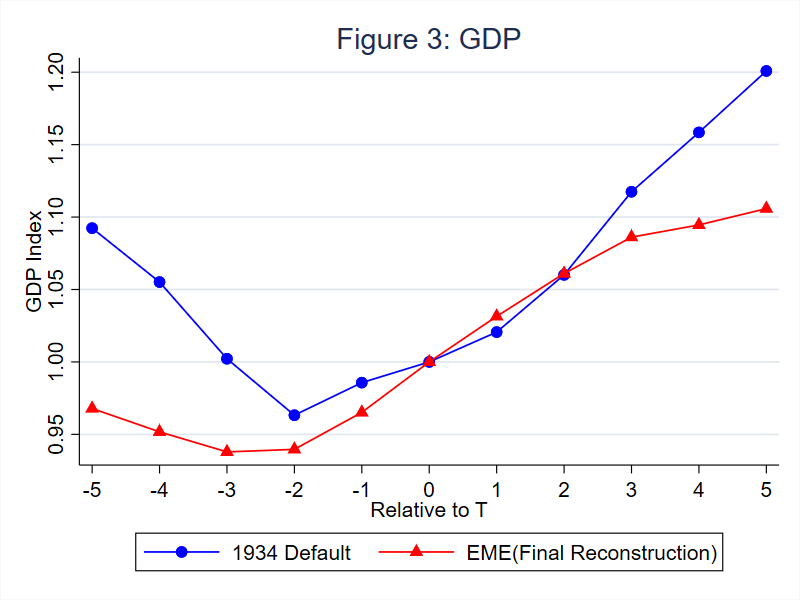
\includegraphics[width=0.9\linewidth]{figures/Figure3_GDP_Comparison.png} % NOTE: Report caption says "Real p.c. GDP" but filename is "GDP_Comparison" - using report caption text for Figure3
      \captionof{figure}{\tiny Real p.c. GDP around debt relief (EM 1978-2010 vs. AE 1934).}
      \label{fig:3_slide}
    \end{column}
    \begin{column}{0.5\textwidth}
      \centering
      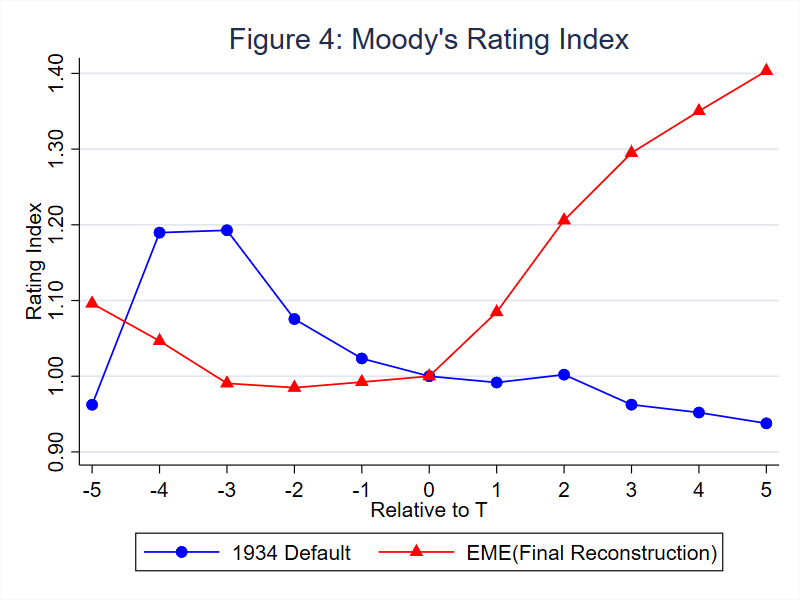
\includegraphics[width=0.9\linewidth]{figures/Figure4_Rating_Comparison.png} % NOTE: Report caption says "Total external debt to GDP" but filename is "Rating_Comparison" - using report caption text for Figure4
      \captionof{figure}{\tiny Total external debt to GDP around debt relief (EM 1978-2010 vs. AE 1934).}
      \label{fig:4_slide}
    \end{column}
  \end{columns}
  \vspace{0.5cm}
  \tiny Report Figure 3 caption: Real per capita GDP around debt relief events (exit from default) in middle- to high- income emerging markets (1978-2010) and advanced economies (1934).
  Report Figure 4 caption: Total external debt to GDP (in \%) around debt relief events (exit from default) in middle- to high-income emerging markets (1978-2010) and advanced economies (1934).
  I used the text caption.
\end{frame}

\begin{frame}{War Period}
  \frametitle{Figure 5 \& 6: Debt Service/GDP and Debt/GDP around Relief}
    \begin{columns}
    \begin{column}{0.5\textwidth}
      \centering
      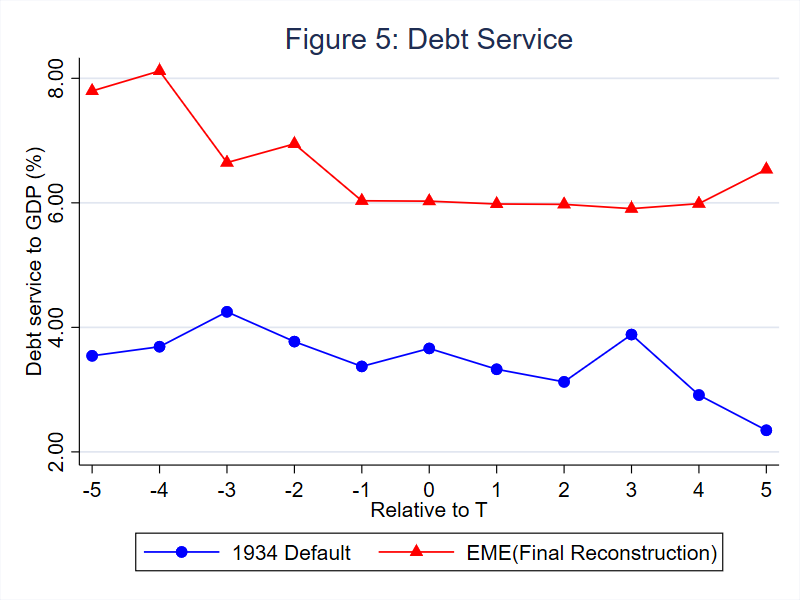
\includegraphics[width=0.9\linewidth]{figures/Figure5_DebtService_Comparison.png}
      \captionof{figure}{\tiny Total debt service to GDP around debt relief (EM 1978-2010 vs AE 1934).}
      \label{fig:5_slide}
    \end{column}
    \begin{column}{0.5\textwidth}
      \centering
      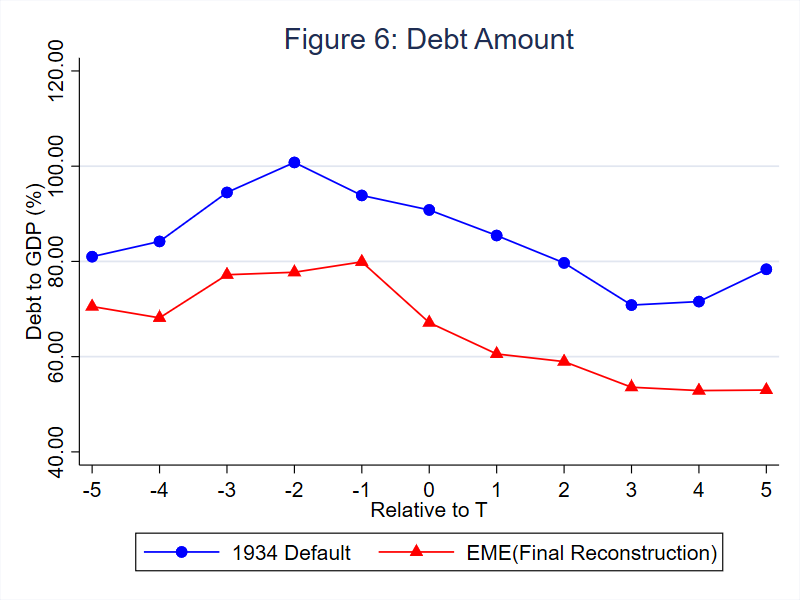
\includegraphics[width=0.9\linewidth]{figures/Figure6_DebtStock_Comparison.png}
      \captionof{figure}{\tiny Debt to GDP around debt relief (EM 1978-2010 vs AE 1934).}
      \label{fig:6_slide}
    \end{column}
  \end{columns}
\end{frame}

\begin{frame}{War Period: DID Analysis - Descriptive Plots}
  \frametitle{DID Analysis: Context - Hoover Moratorium 1931}
  \begin{itemize}
    \item Brady target group: Various EMs (Argentina, Brazil, etc.).
    \item Baker sample: Similar to Brady, and Chile.
    \item Baseline counterfactual: Middle/high-income non-defaulters (China, Colombia, etc.).
  \end{itemize}
  \centering
  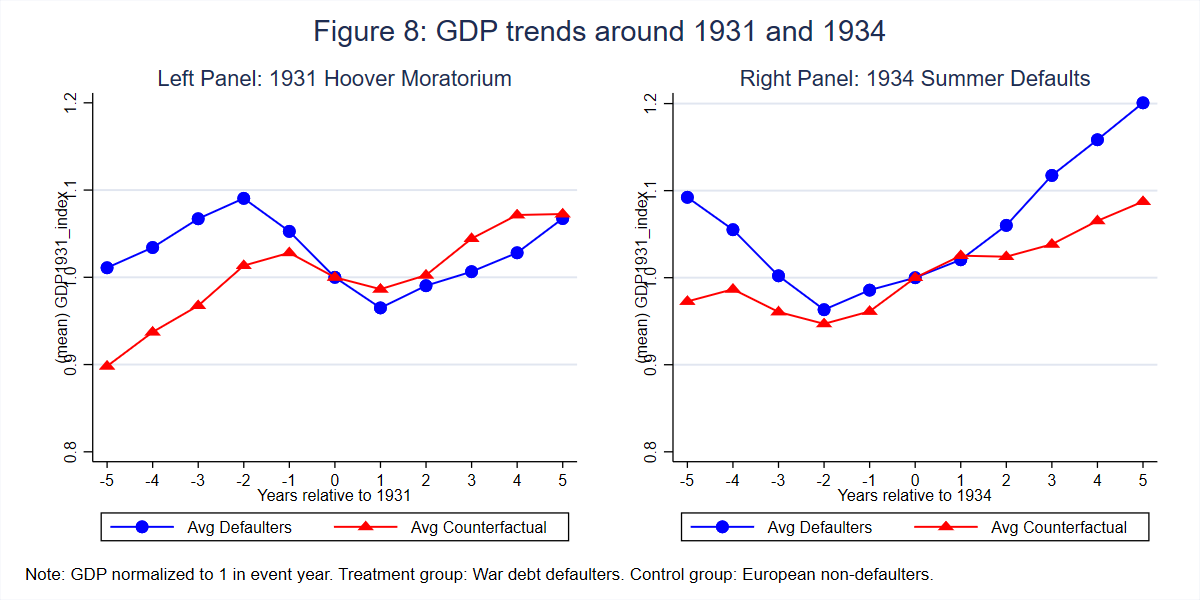
\includegraphics[width=0.7\linewidth]{figures/Figure8_GDP_trends_1931_1934.png}
  \captionof{figure}{\tiny GDP trends around 1931 and 1934.}
  \label{fig:8_slide}
\end{frame}

\begin{frame}{War Period: DID Analysis - Indicator Comparison (Fig C5)}
  \frametitle{Economic Indicators: Treatment vs. Control (Europe Non-Defaulters)}
  \begin{columns}[T] % T for top alignment
    \begin{column}{0.45\textwidth}
      \centering
      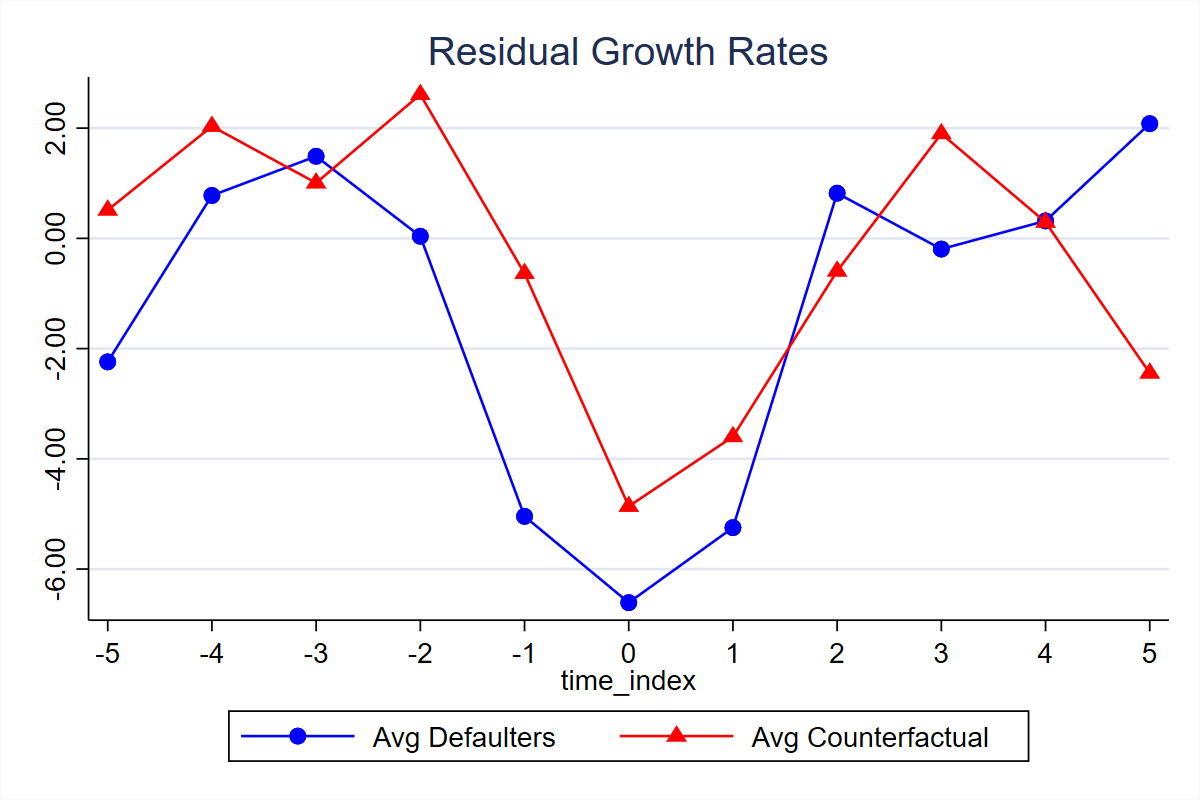
\includegraphics[width=0.9\linewidth]{figures/figc5_a.png}
      % \captionof{figure}{\tiny Residual GDP Growth}
      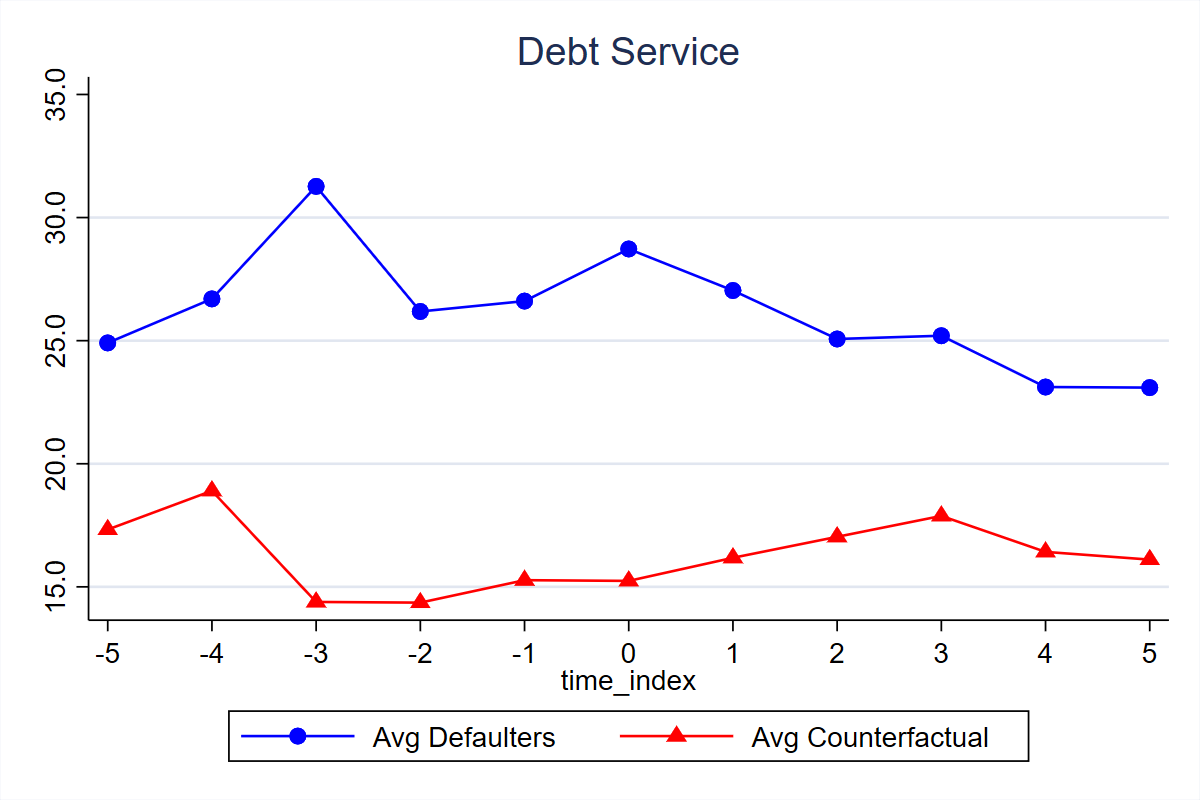
\includegraphics[width=0.9\linewidth]{figures/figc5_c.png}
      % \captionof{figure}{\tiny Debt Service to Revenue}
    \end{column}
    \begin{column}{0.45\textwidth}
      \centering
      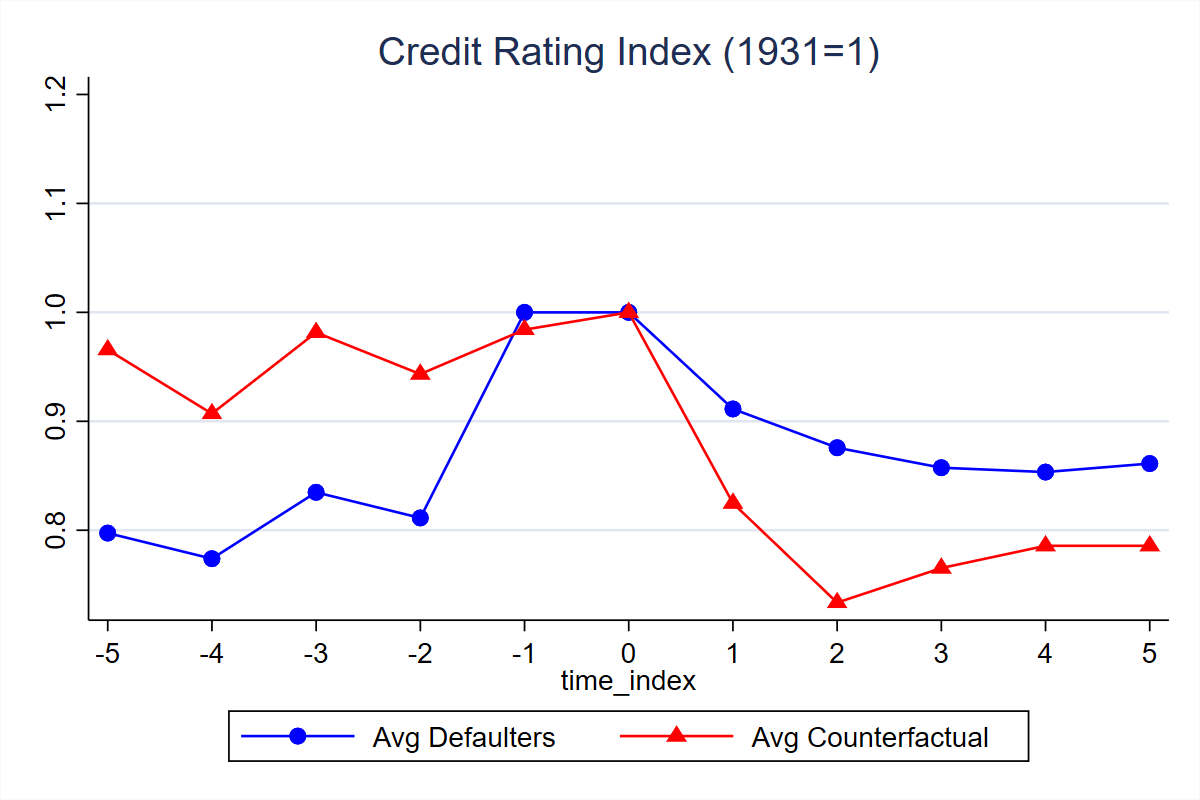
\includegraphics[width=0.9\linewidth]{figures/figc5_b.png}
      % \captionof{figure}{\tiny Credit Ratings}
      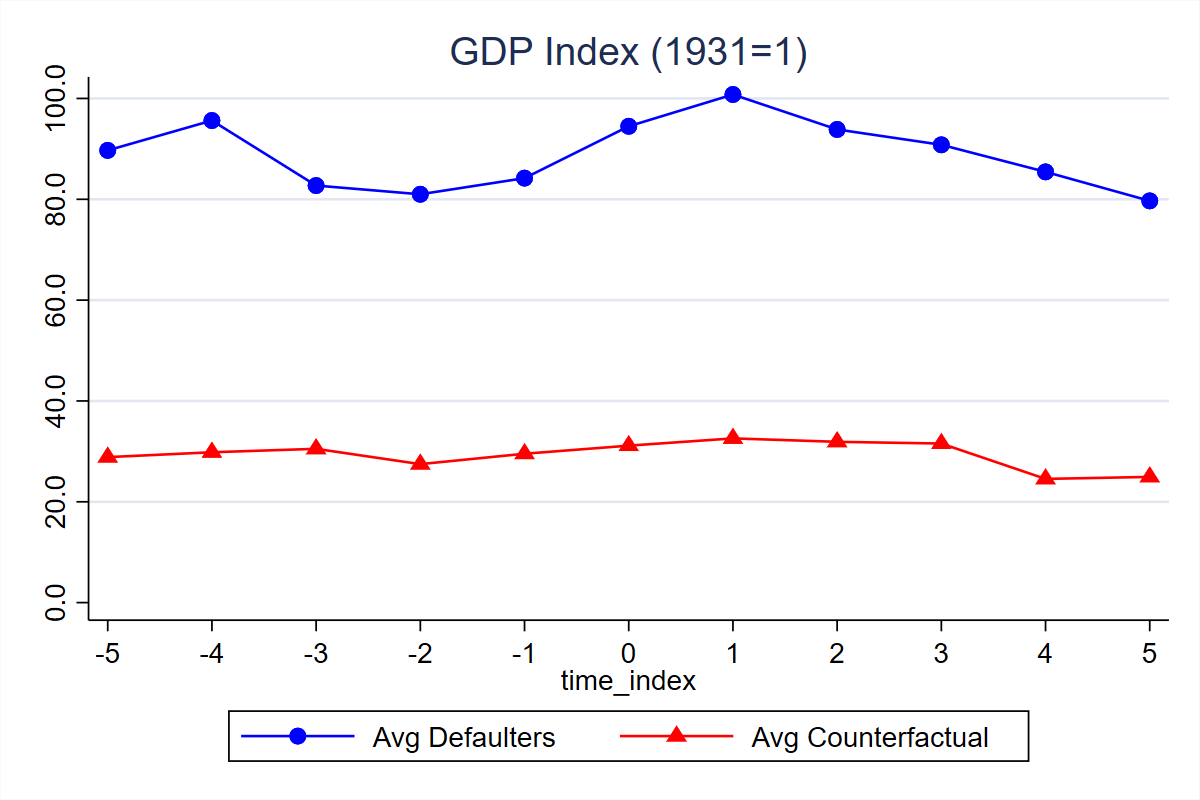
\includegraphics[width=0.9\linewidth]{figures/figc5_d.png}
      % \captionof{figure}{\tiny Debt to GDP}
    \end{column}
  \end{columns}
  \tiny \textbf{Summary for 1931}: Treatment group growth worse. Residual growth declines for both, recovers, no better performance for treatment. Ratings decline across board. Debt/GDP no significant difference. Debt servicing improves more for treatment.
\end{frame}

\begin{frame}{War Period: Parallel Trend Test}
  \frametitle{Parallel Trend Test (Self-Conducted)}
  We conducted parallel trend tests since the original paper only performed descriptive analysis.
  \begin{itemize}
    \item \textbf{Key Findings}:
    \begin{itemize}
        \item Most variables passed the parallel trend assumption.
        \item \alert{Interpret with caution for}:
        \begin{itemize}
            \item Credit rating results for 1934.
            \item Debt/GDP ratio and external debt/GDP ratio results for 1931.
        \end{itemize}
    \end{itemize}
  \end{itemize}
  % \textit{(The presentation would ideally show key graphs or a summary table from the PT tests. The report includes 12 PT figures; select a few representative ones.)}
  \begin{columns}
    \begin{column}{0.5\textwidth}
      \centering 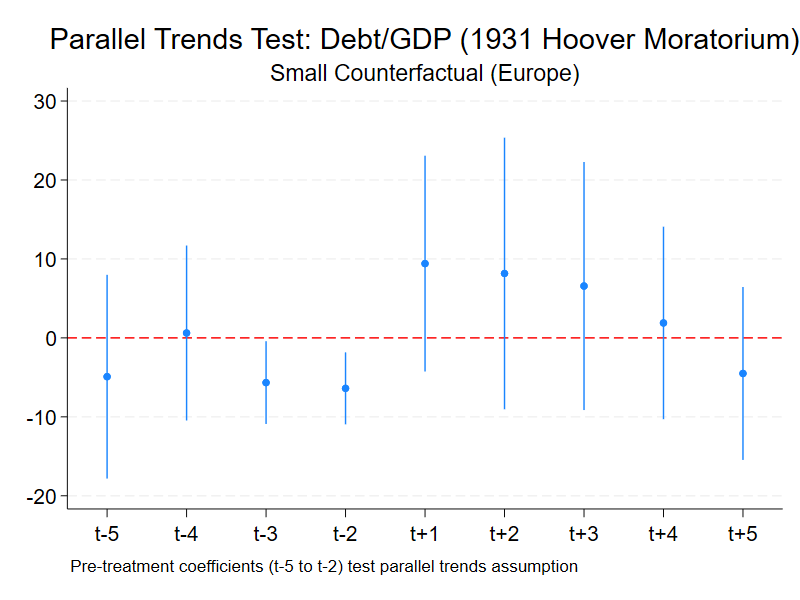
\includegraphics[width=0.8\linewidth]{figures/PT_Debt_1931_Small.png} 
      % \captionof{figure}{\tiny PT: Debt 1934 Small Sample}
    \end{column}
    \begin{column}{0.5\textwidth}
      \centering 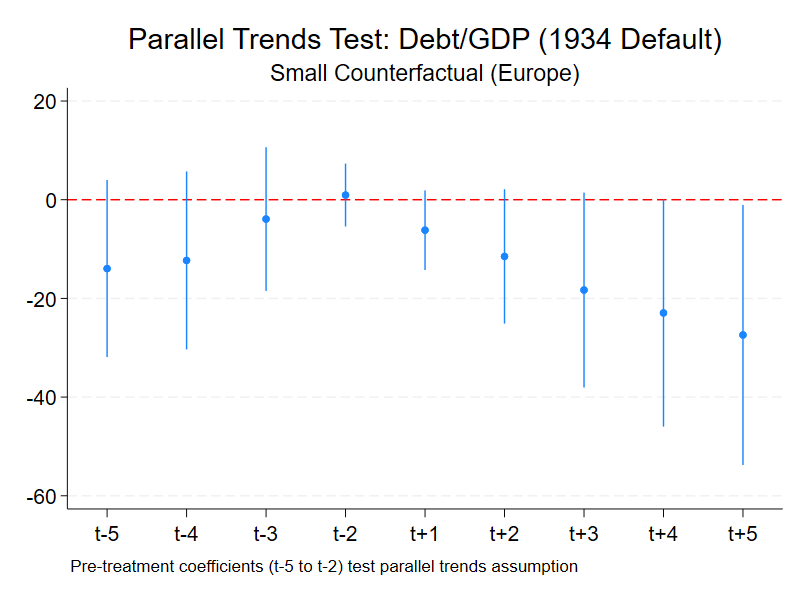
\includegraphics[width=0.8\linewidth]{figures/PT_Debt_1934_Small.png} 
      % \captionof{figure}{\tiny PT: GDP 1934 Small Sample}
    \end{column}
  \end{columns}
\end{frame}

\begin{frame}{War Period: Parallel Trend Test (Cont'd)}
  \frametitle{Parallel Trend Test (Cont'd)}
  \begin{columns}[T] % T for top alignment
    \begin{column}{0.45\textwidth}
      \centering
      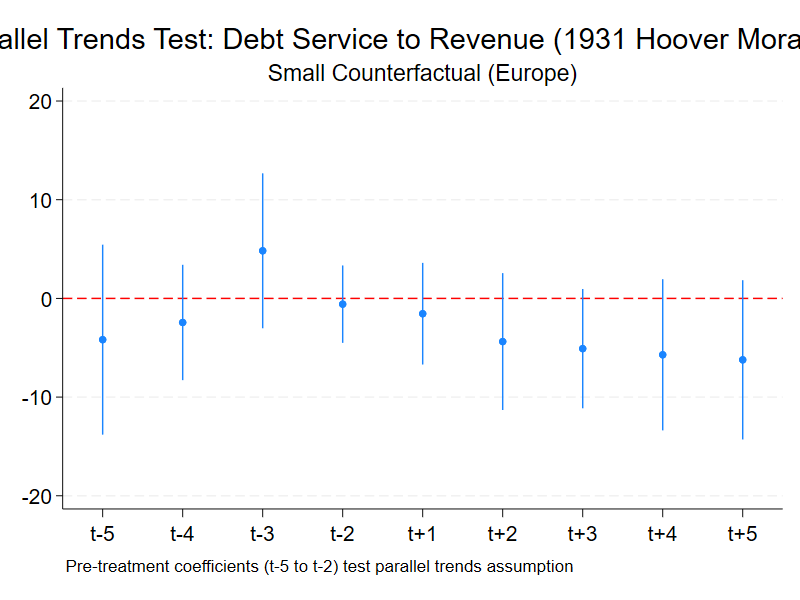
\includegraphics[width=0.9\linewidth]{figures/PT_DebtServ_1931_Small.png}
      % \captionof{figure}{\tiny PT: Baker Rating}
      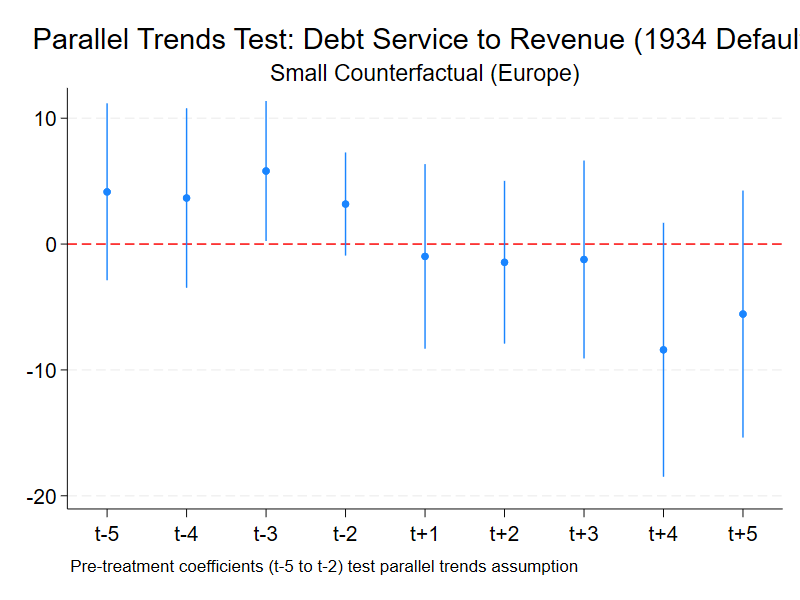
\includegraphics[width=0.9\linewidth]{figures/PT_DebtServ_1934_Small.png}
    \end{column}
    \begin{column}{0.45\textwidth}
      \centering
      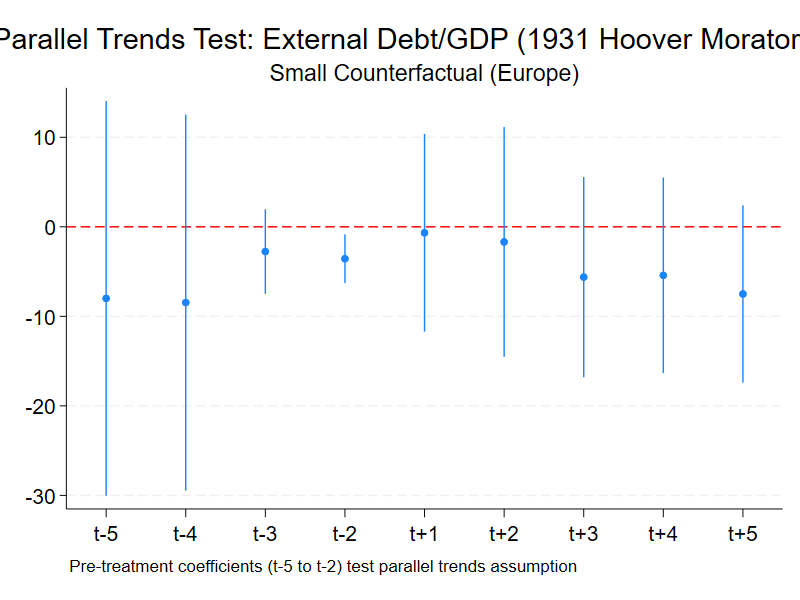
\includegraphics[width=0.9\linewidth]{figures/PT_ExtDebt_1931.png}
      % \captionof{figure}{\tiny PT: Brady Rating}
      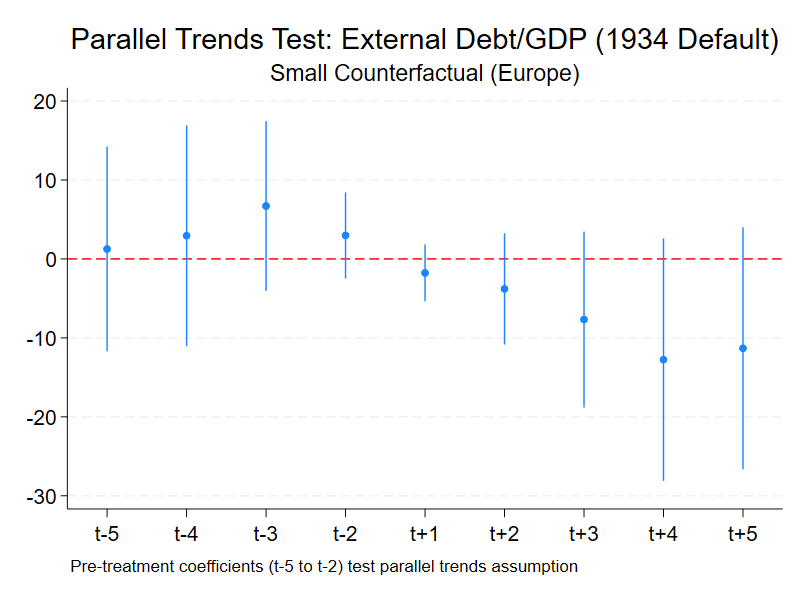
\includegraphics[width=0.9\linewidth]{figures/PT_ExtDebt_1934.png}
    \end{column}
  \end{columns}
\end{frame}

\begin{frame}{War Period: Parallel Trend Test (Cont'd)}
  \frametitle{Parallel Trend Test (Cont'd)}
  \begin{columns}[T] % T for top alignment
    \begin{column}{0.45\textwidth}
      \centering
      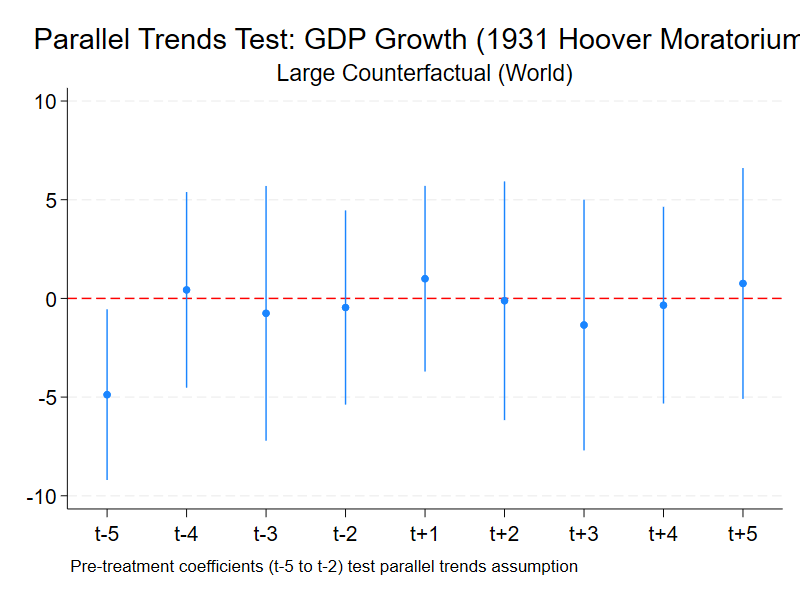
\includegraphics[width=0.9\linewidth]{figures/PT_GDP_1931_Large.png}
      % \captionof{figure}{\tiny PT: Baker Rating}
      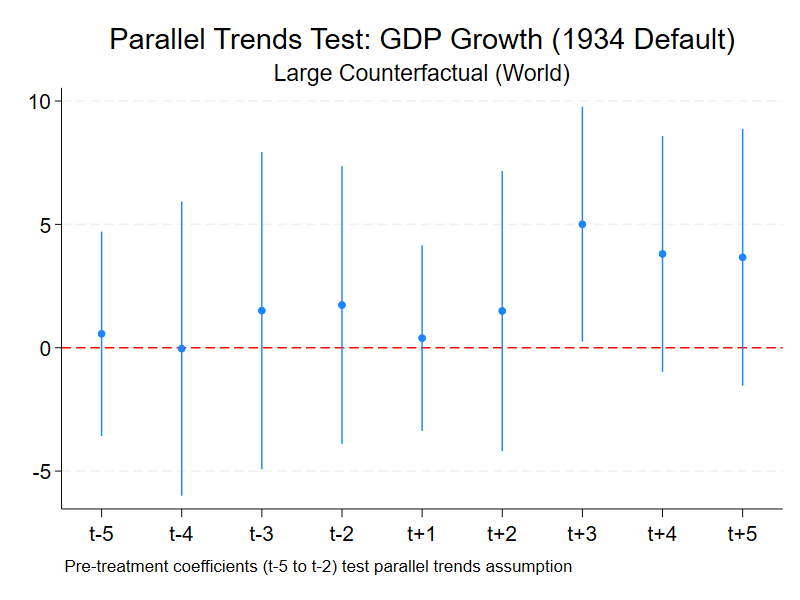
\includegraphics[width=0.9\linewidth]{figures/PT_GDP_1934_Large.png}
    \end{column}
    \begin{column}{0.45\textwidth}
      \centering
      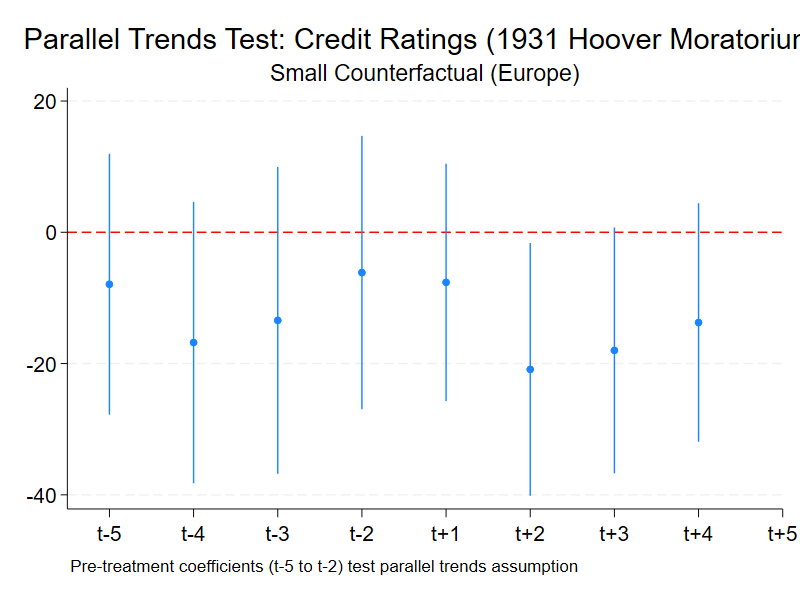
\includegraphics[width=0.9\linewidth]{figures/PT_Ratings_1931.png}
      % \captionof{figure}{\tiny PT: Brady Rating}
      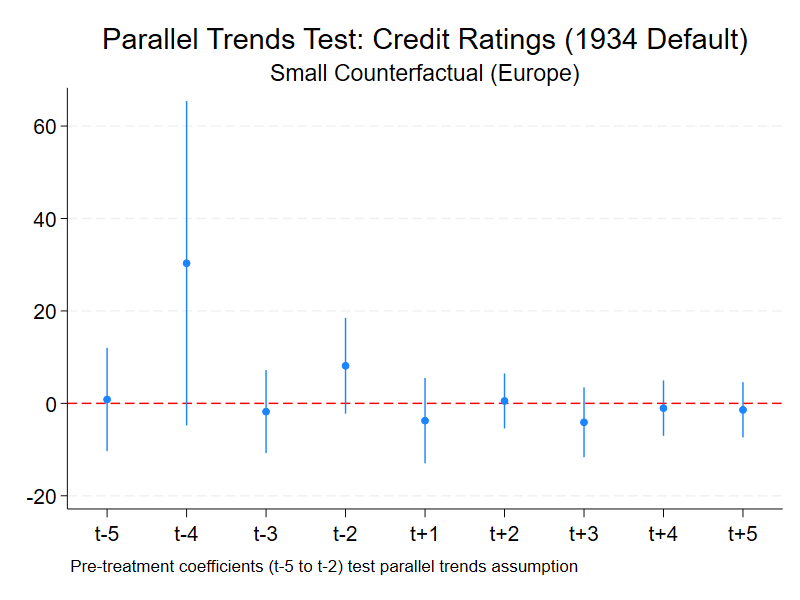
\includegraphics[width=0.9\linewidth]{figures/PT_Ratings_1934.png}
    \end{column}
  \end{columns}
\end{frame}

\begin{frame}{War Period: Parallel Trend Test (Cont'd)}
  \frametitle{Parallel Trend Test (Cont'd)}
  \begin{columns}[T] % T for top alignment
    \begin{column}{0.45\textwidth}
      \centering
      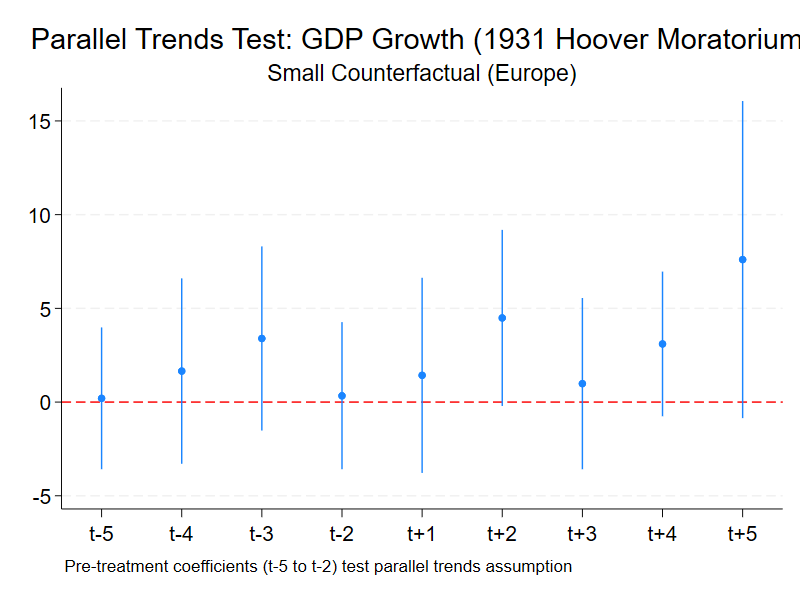
\includegraphics[width=0.9\linewidth]{figures/PT_GDP_1931_Small.png}
      % \captionof{figure}{\tiny PT: Baker Rating}
    \end{column}
    \begin{column}{0.45\textwidth}
      \centering
      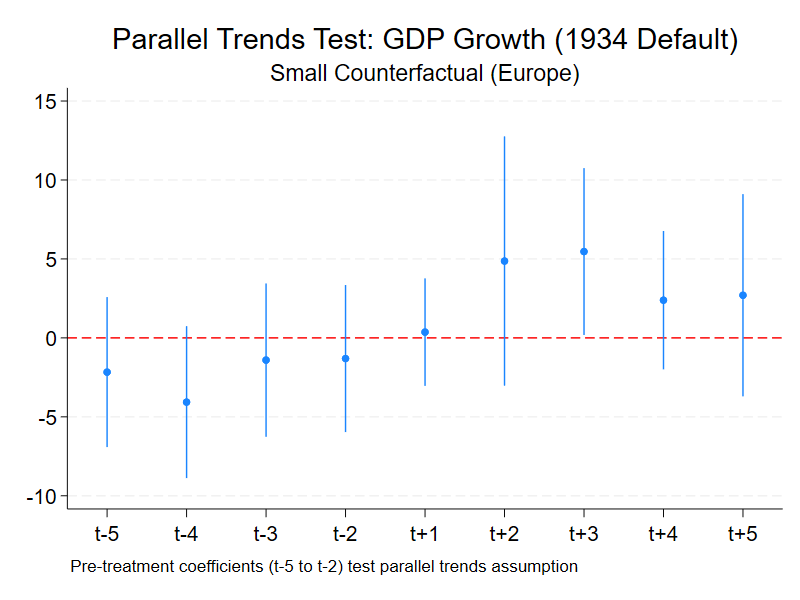
\includegraphics[width=0.9\linewidth]{figures/PT_GDP_1934_Small.png}
      % \captionof{figure}{\tiny PT: Brady Rating}
    \end{column}
  \end{columns}
\end{frame}

\begin{frame}{War period: PT Test}
    \begin{table}[ht!]
\centering
\begin{tabular}{lccc}
\toprule
Variable & P‐Value & Pass (5\%) & Pass (10\%) \\
\midrule
GDP\_Growth\_1934\_l   & 0.52529567 & 1 & 1 \\
GDP\_Growth\_1934\_e   & 0.94559858 & 1 & 1 \\
Ratings\_1934          & 0.04996219 & 0 & 0 \\
DebtServ\_1934\_l      & 0.13978740 & 1 & 1 \\
DebtServ\_1934\_e      & 0.51155188 & 1 & 1 \\
Debt\_GDP\_1934\_l     & 0.12776463 & 1 & 1 \\
Debt\_GDP\_1934\_e     & 0.25006164 & 1 & 1 \\
ExtDebt\_1934          & 0.06999843 & 1 & 0 \\
\midrule
GDP\_Growth\_1931\_l   & 0.57373095 & 1 & 1 \\
GDP\_Growth\_1931\_e   & 0.23592213 & 1 & 1 \\
Ratings\_1931          & 0.41062027 & 1 & 1 \\
DebtServ\_1931\_l      & 0.28772333 & 1 & 1 \\
DebtServ\_1931\_e      & 0.39504800 & 1 & 1 \\
Debt\_GDP\_1931\_l     & 0.01403155 & 0 & 0 \\
Debt\_GDP\_1931\_e     & 0.07416818 & 1 & 0 \\
ExtDebt\_1931          & 0.01362215 & 0 & 0 \\
\bottomrule
\end{tabular}
\caption{P-values and pass/fail indicators at 5\% and 10\% levels}
\label{tab:pass_tests}
\end{table}

\end{frame}

\begin{frame}{Table 3 1931 Hoover Replication}
  \begin{figure}
      \centering
      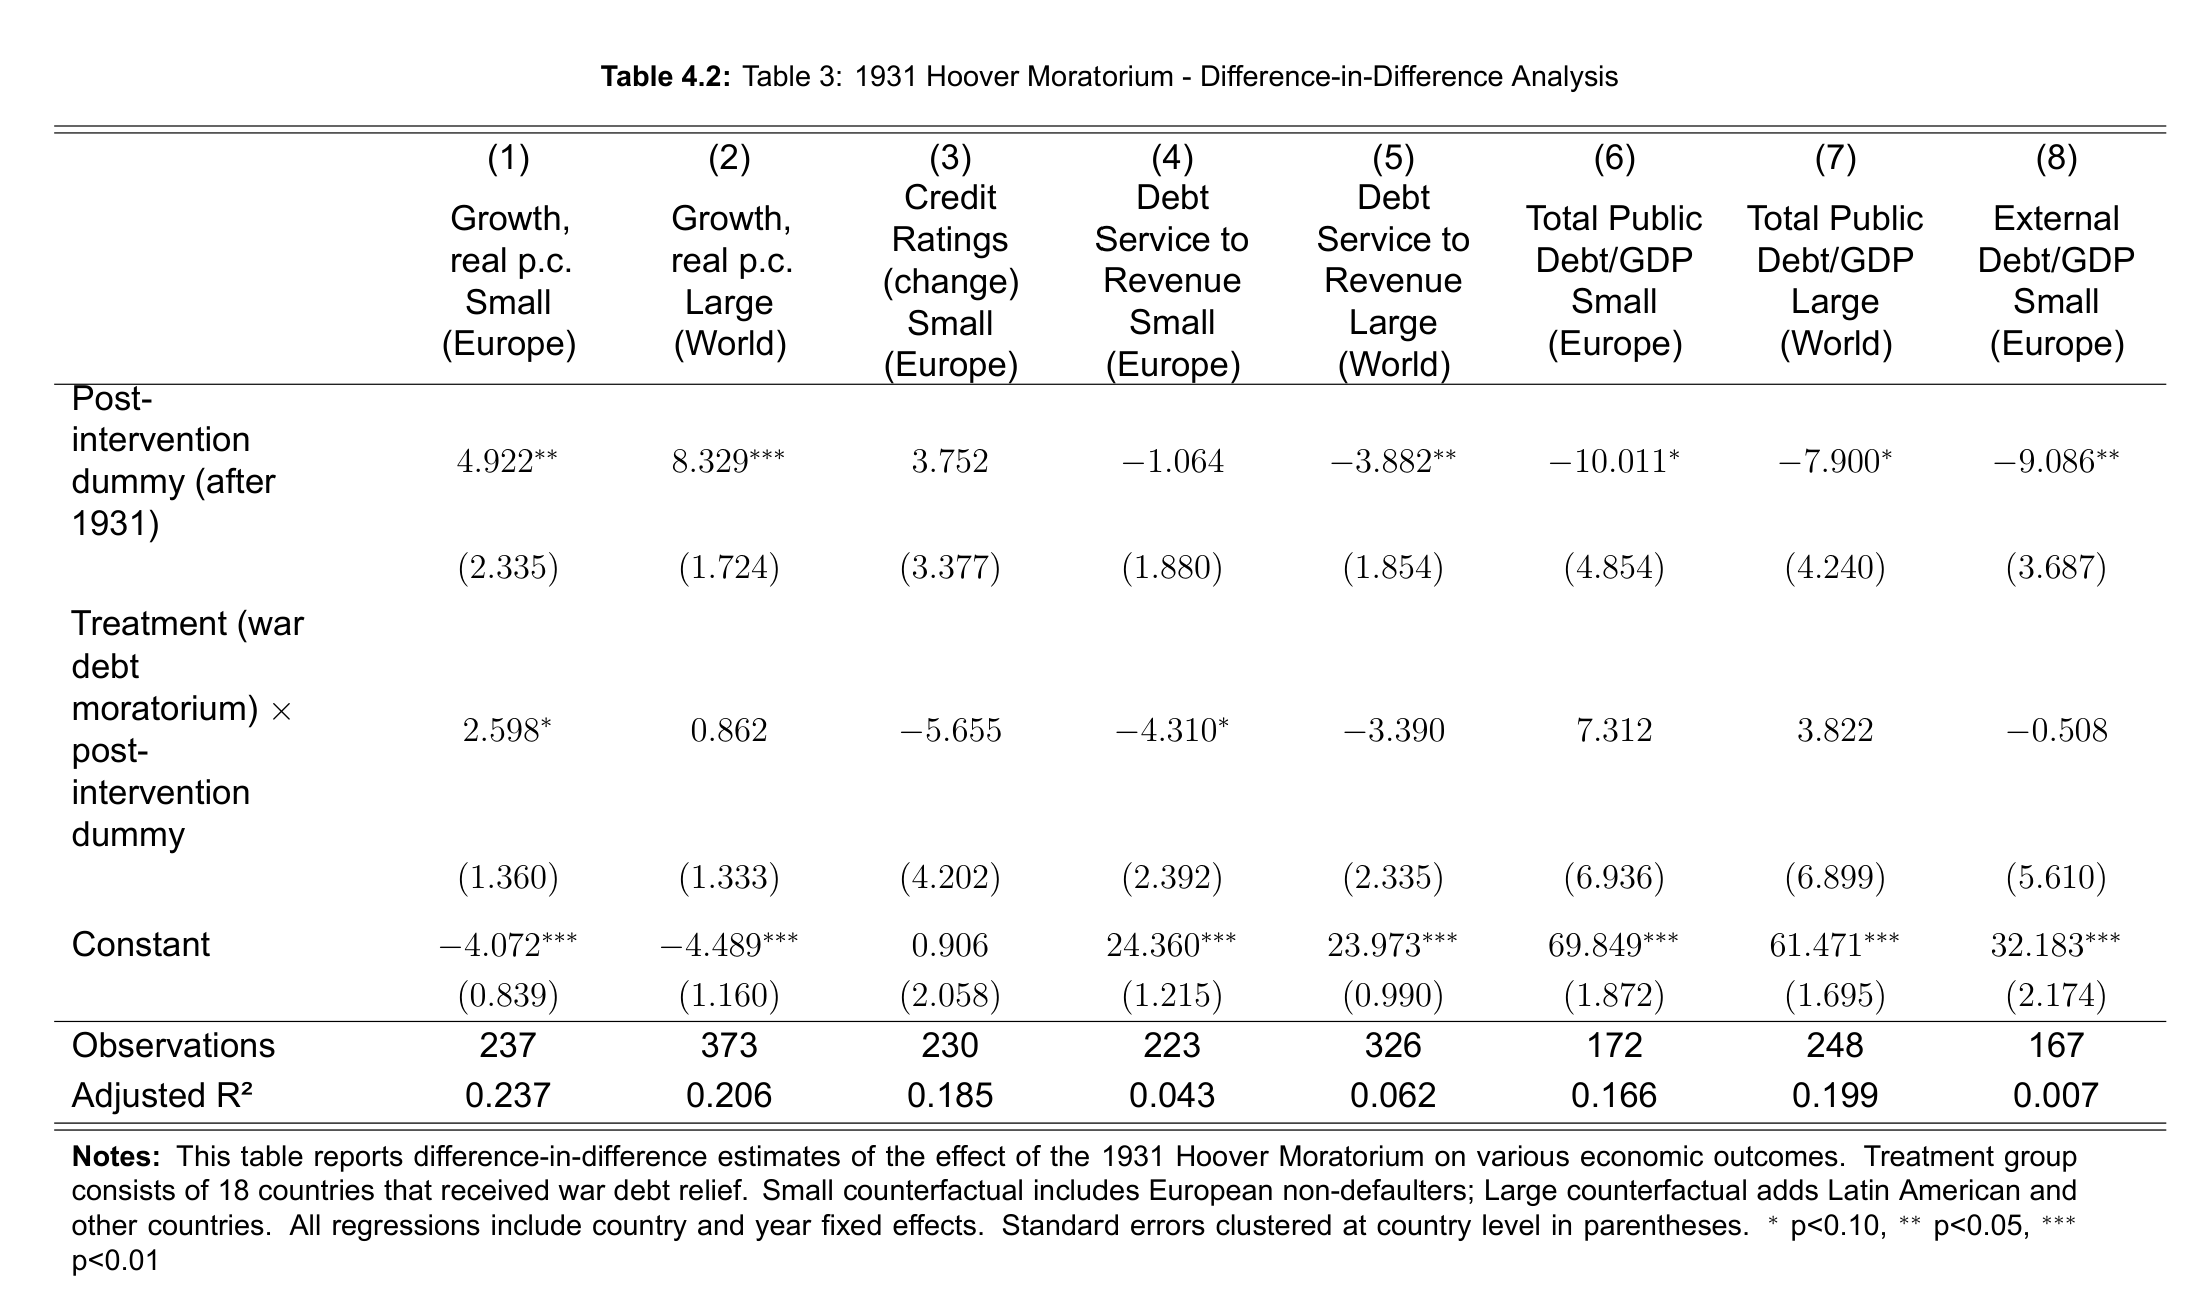
\includegraphics[width=0.95\linewidth]{figures/tab3_rep.png}
      \captionof{figure}{\tiny Table 3: Replication of 1931 Hoover Moratorium Results}
      \label{fig:table3_1931}
  \end{figure}
\end{frame}

\begin{frame}{Table 3 Replication: Visual Evidence}
  \frametitle{Comparison: Published vs. Replicated Results}
  \begin{figure}
      \centering
      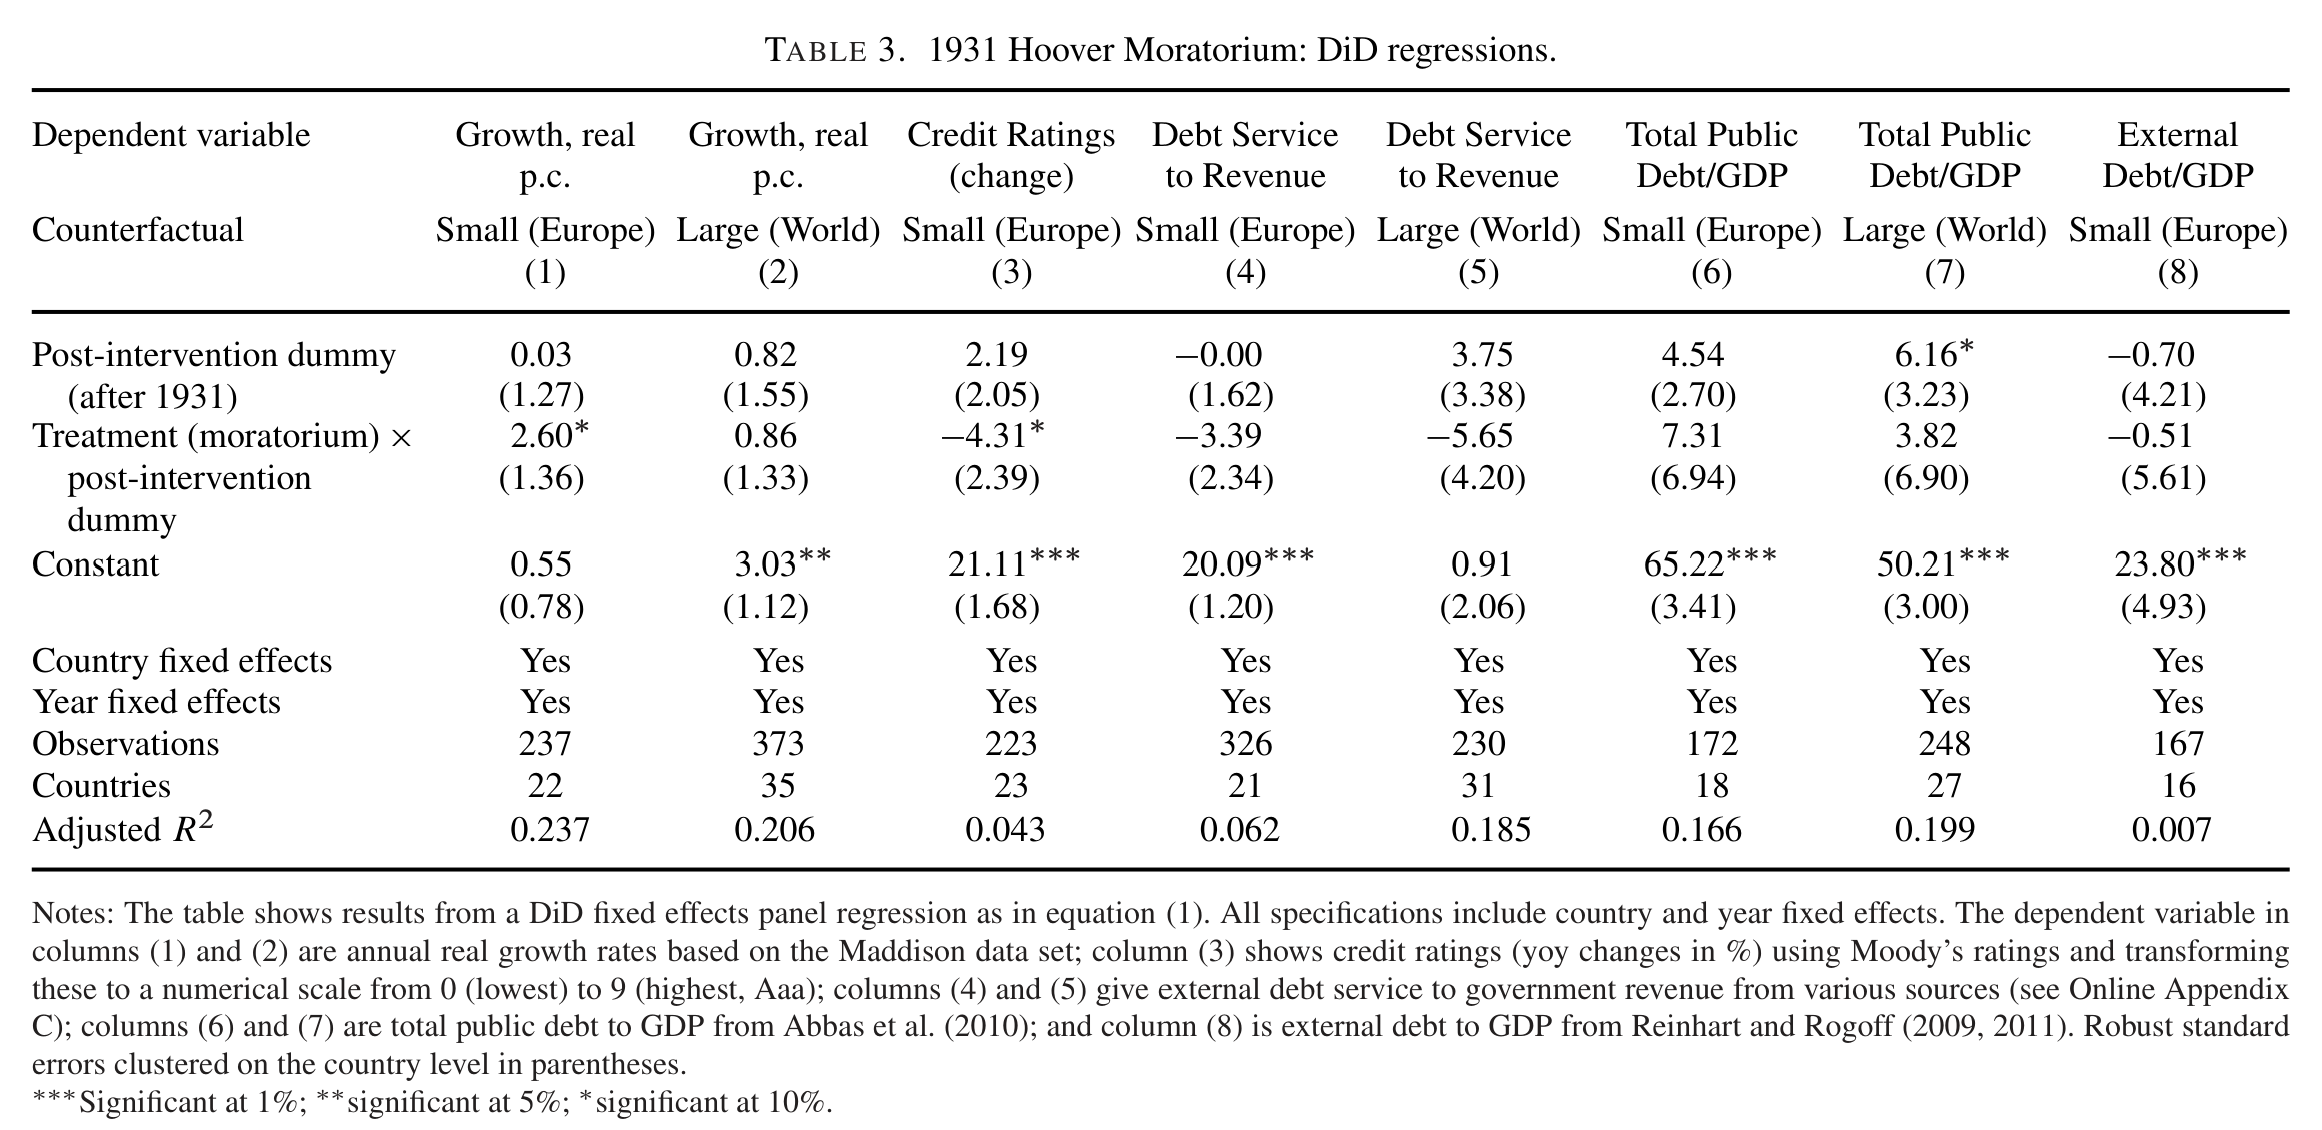
\includegraphics[width=0.95\linewidth]{figures/table3_original.png}
      % \captionof{figure}{\tiny Table 3 (Published Results)}
  \end{figure}
  \begin{itemize}
    \item \textbf{Key Observation}: Substantial differences in coefficient magnitudes and significance levels
    \item \textbf{Implication}: Results interpretation and economic conclusions may need revision
  \end{itemize}
\end{frame}

\begin{frame}{Table 3 Replication: Data Inconsistencies Found}
  \frametitle{Major Discrepancies in Table 3 Results}
  \begin{itemize}
    \item \textbf{Column Order Issue}:
    \begin{itemize}
        \item Original Table 3 columns (3), (4), (5) appear to be in wrong order
        \item Correct data order should be: (5), (3), (4)
        \item This affects interpretation of debt service and debt level results
    \end{itemize}
    \item \textbf{Post-intervention Dummy Coefficients}:
    \begin{itemize}
        \item Our replicated "after 1931" coefficients differ substantially from published results
        \item Issue persists even when dropping year fixed effects
        \item \alert{Authors' original code produces same results as our replication, not published table}
    \end{itemize}
    \item \textbf{Statistical Significance Mismatch}:
    \begin{itemize}
        \item Authors claim: "Only $\beta_2$ coefficients marginally significant are GDP and credit ratings"
        \item Our results: Only credit ratings and debt service to revenue are \textit{insignificant}
        \item This is a fundamental contradiction in interpretation
    \end{itemize}
  \end{itemize}
\end{frame}

\begin{frame}{Table 3 Replication: Detailed Coefficient Comparison}
  \frametitle{Column 4 Detailed Analysis}
  \begin{columns}
    \begin{column}{0.5\textwidth}
      \centering
      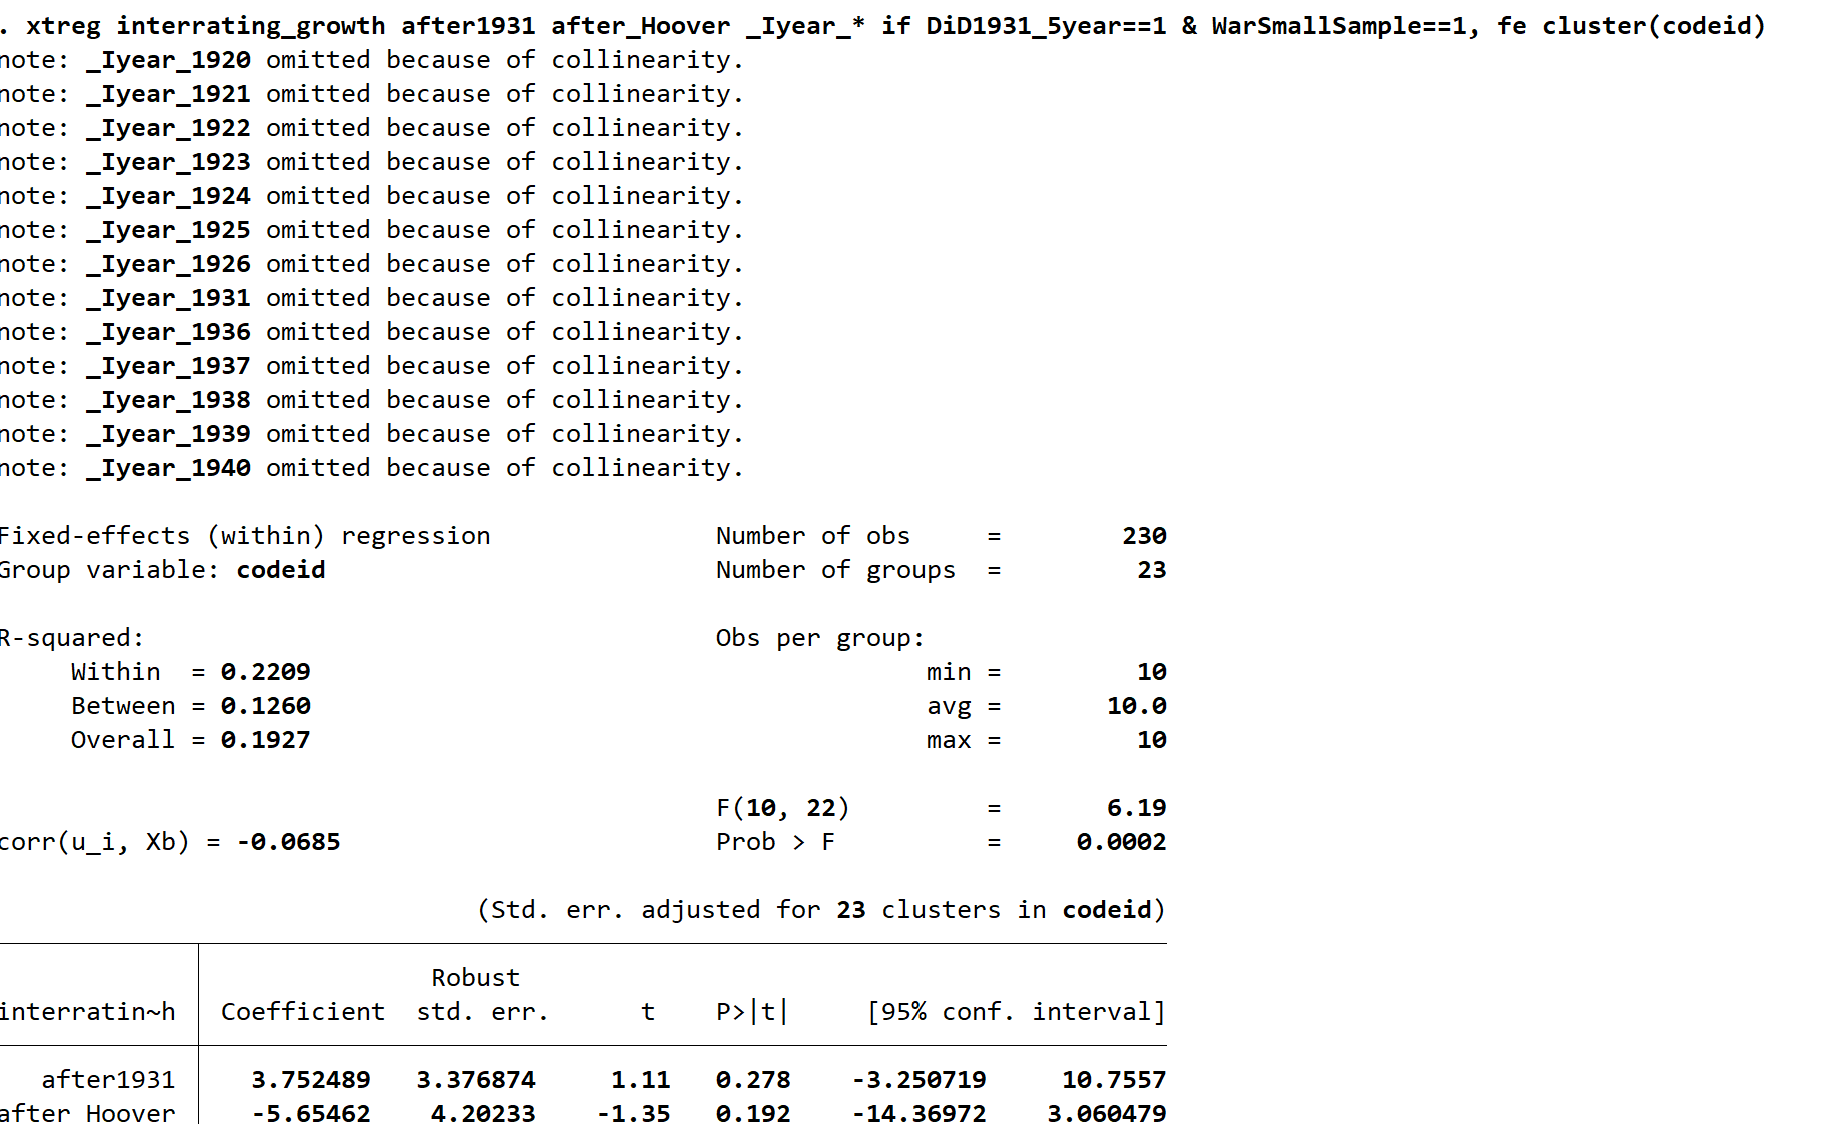
\includegraphics[width=0.95\linewidth]{figures/col3_tab3_stata.png}
      \captionof{figure}{\tiny Table 3 Col 3 (Our Replication)}
      \label{fig:table3_col3}
    \end{column}
    \begin{column}{0.5\textwidth}
      \centering
      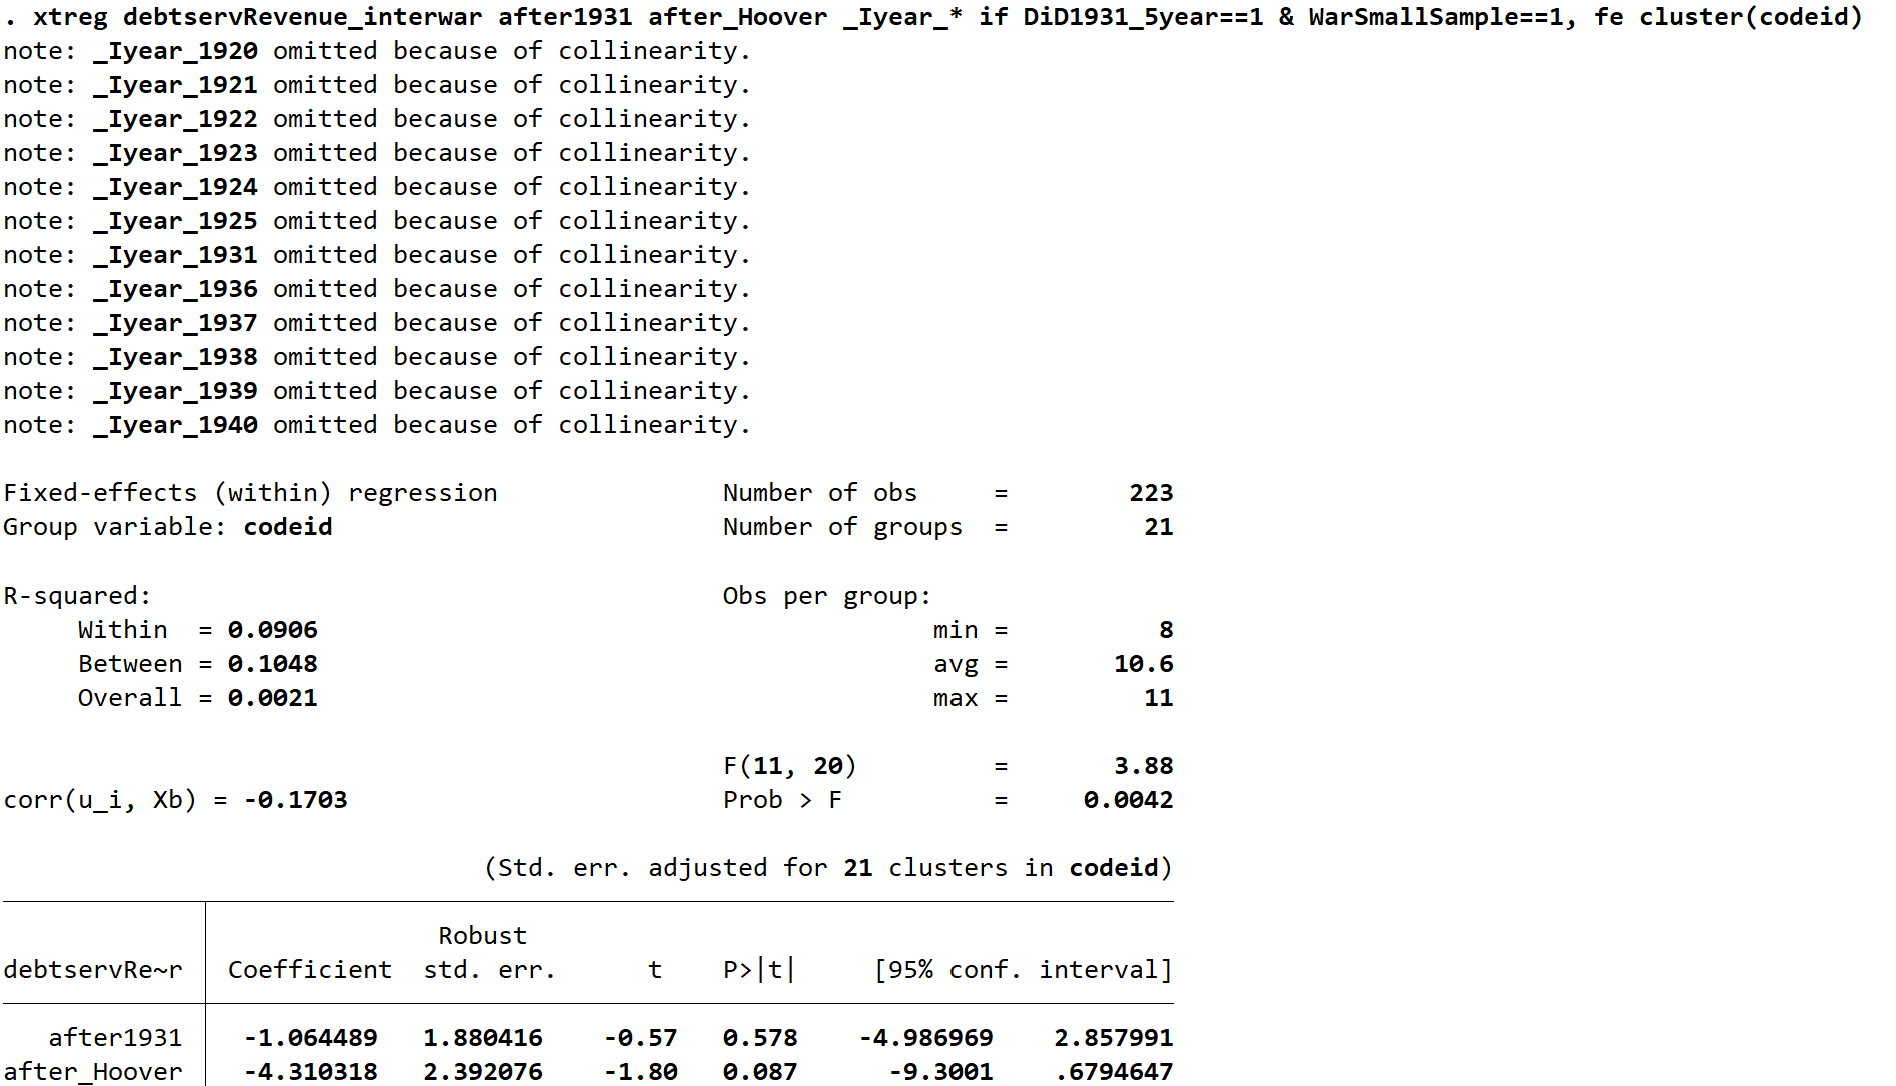
\includegraphics[width=0.95\linewidth]{figures/col4_tab3_stata.png}
      \captionof{figure}{\tiny Table 3 Col 4 (Our Replication)}
      \label{fig:table3_col4}
    \end{column}
  \end{columns}
  
  \vspace{0.5cm}
  \begin{itemize}
    \item \textbf{Critical Finding}: Running authors' \textit{original code} reproduces our results, not the published table
    \item \textbf{Methodological Concern}: Suggests potential data processing or reporting errors in original paper
    \item \textbf{Research Integrity}: Highlights importance of code and data transparency in replication studies
  \end{itemize}
\end{frame}

\begin{frame}{Table 3 Replication: Implications for 1931 Hoover Moratorium Analysis}
  \frametitle{Impact on Economic Interpretation}
  \textbf{Original Paper Claims vs. Our Findings:}
  \begin{itemize}
    \item \textbf{Authors' Interpretation}:
    \begin{itemize}
        \item Limited significant effects from 1931 moratorium
        \item Only GDP growth and credit ratings show marginal significance
    \end{itemize}
    \item \textbf{Our Replication Findings}:
    \begin{itemize}
        \item \textcolor{red}{Broader pattern of significant effects}
        \item Multiple debt-related variables show statistical significance
        \item Suggests more substantial impact of 1931 intervention than originally concluded
    \end{itemize}
    \item \textbf{Research Implications}:
    \begin{itemize}
        \item \alert{Calls into question} the paper's conclusions about 1931 vs. 1934 effectiveness
        % \item May require \textbf{reassessment} of historical narrative about debt relief timing
        \item Emphasizes need for \textbf{robust replication practices} in economic history
    \end{itemize}
  \end{itemize}
\end{frame}

\begin{frame}{War Period: Results of DID}
  \frametitle{Results of DID: 1934 Debt Relief Replication}
  \begin{figure}[ht!]
      \centering
      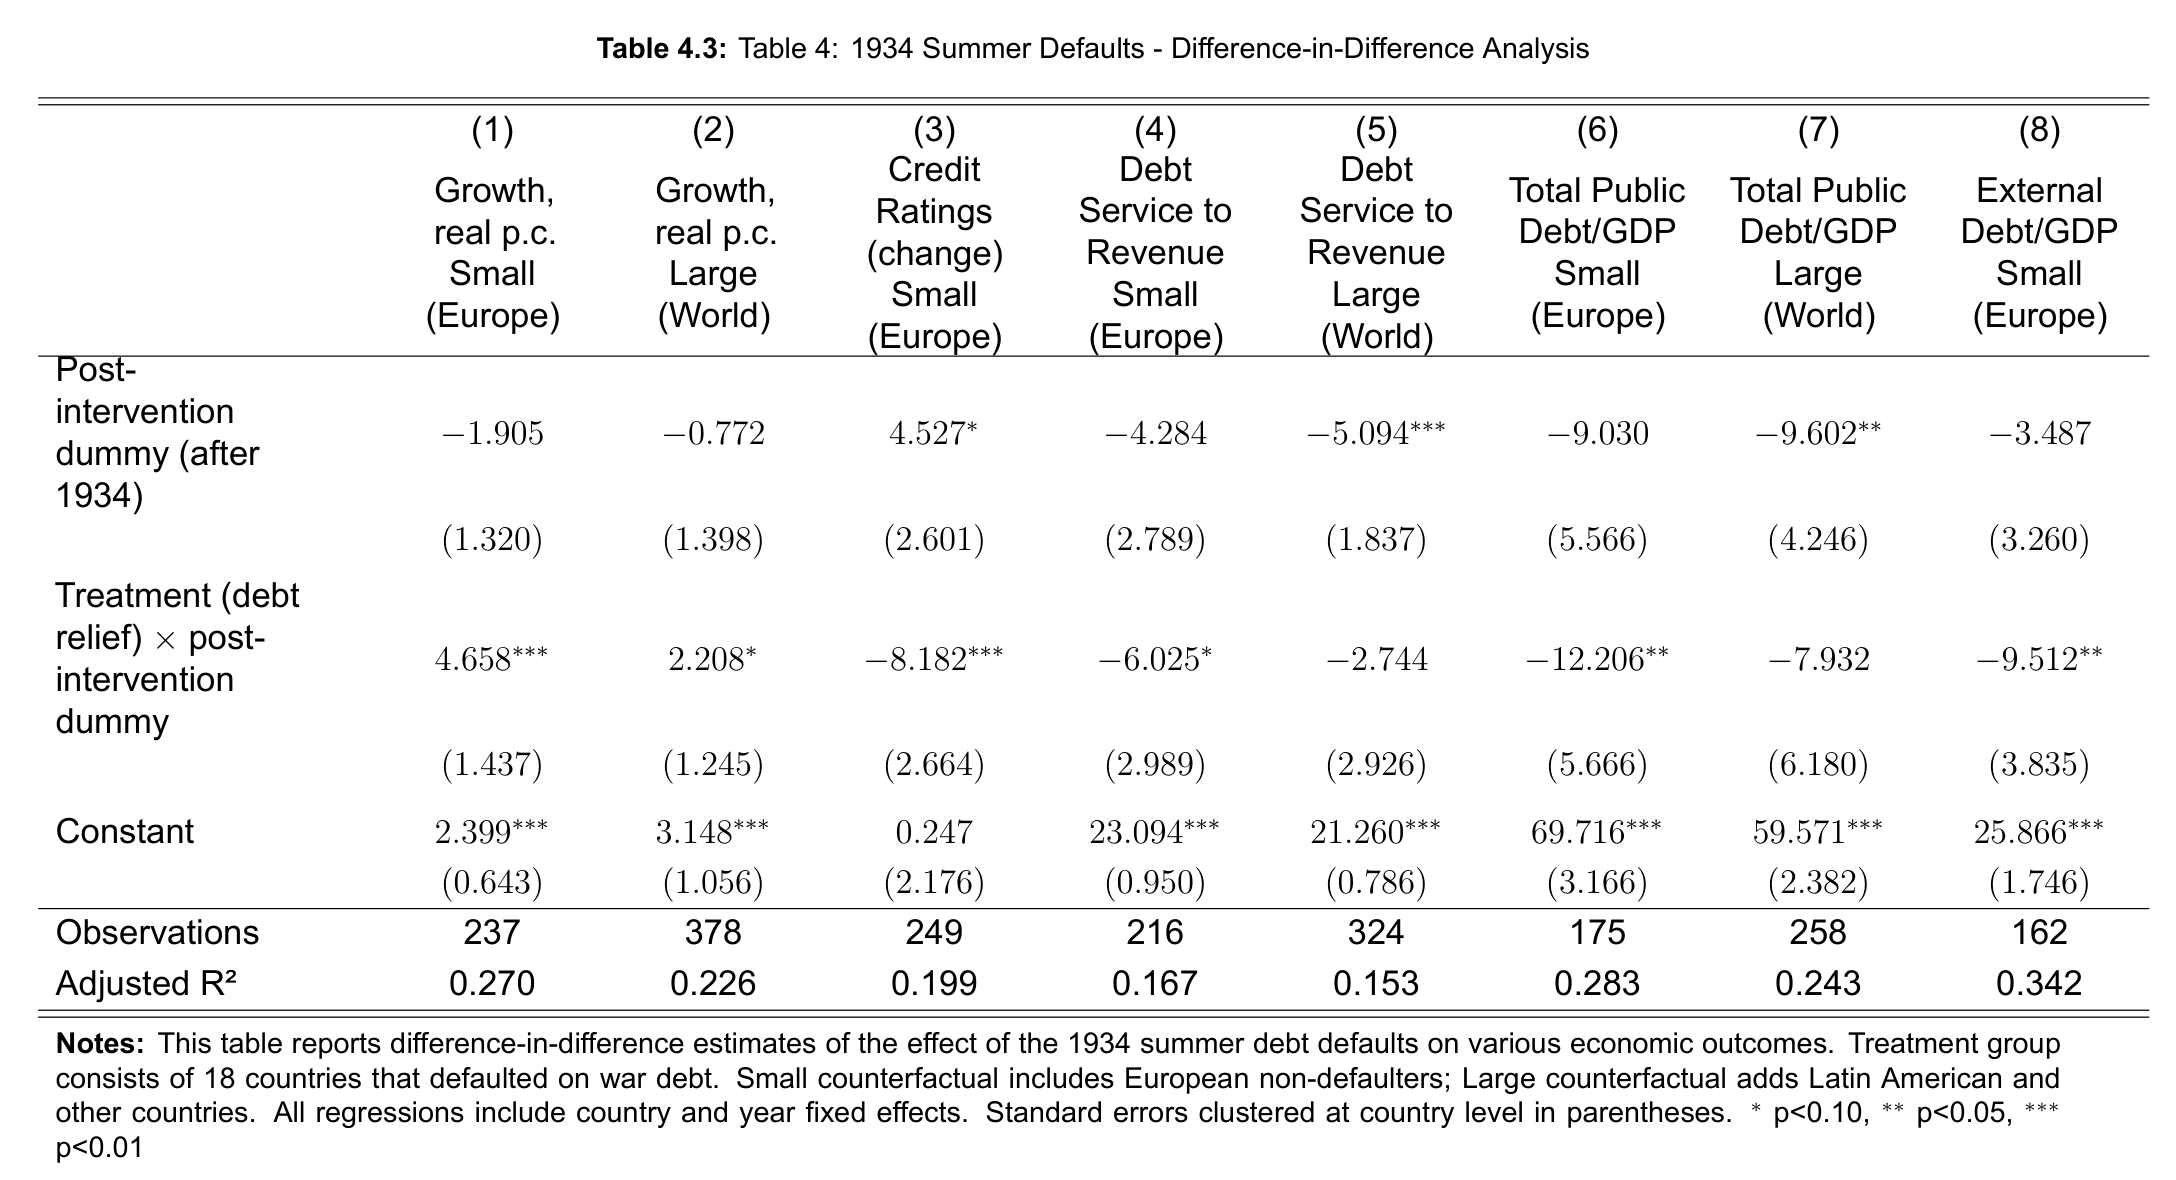
\includegraphics[width=0.95\linewidth]{figures/tab4_rep.png}
      \captionof{figure}{\tiny Replication of 1934 Debt Relief Results}
      \label{fig:tab4_rep}
  \end{figure}  
\end{frame}

\begin{frame}
    \frametitle{Results of DID: 1934 Debt Relief Replication}
  \begin{figure}[ht!]
      \centering
      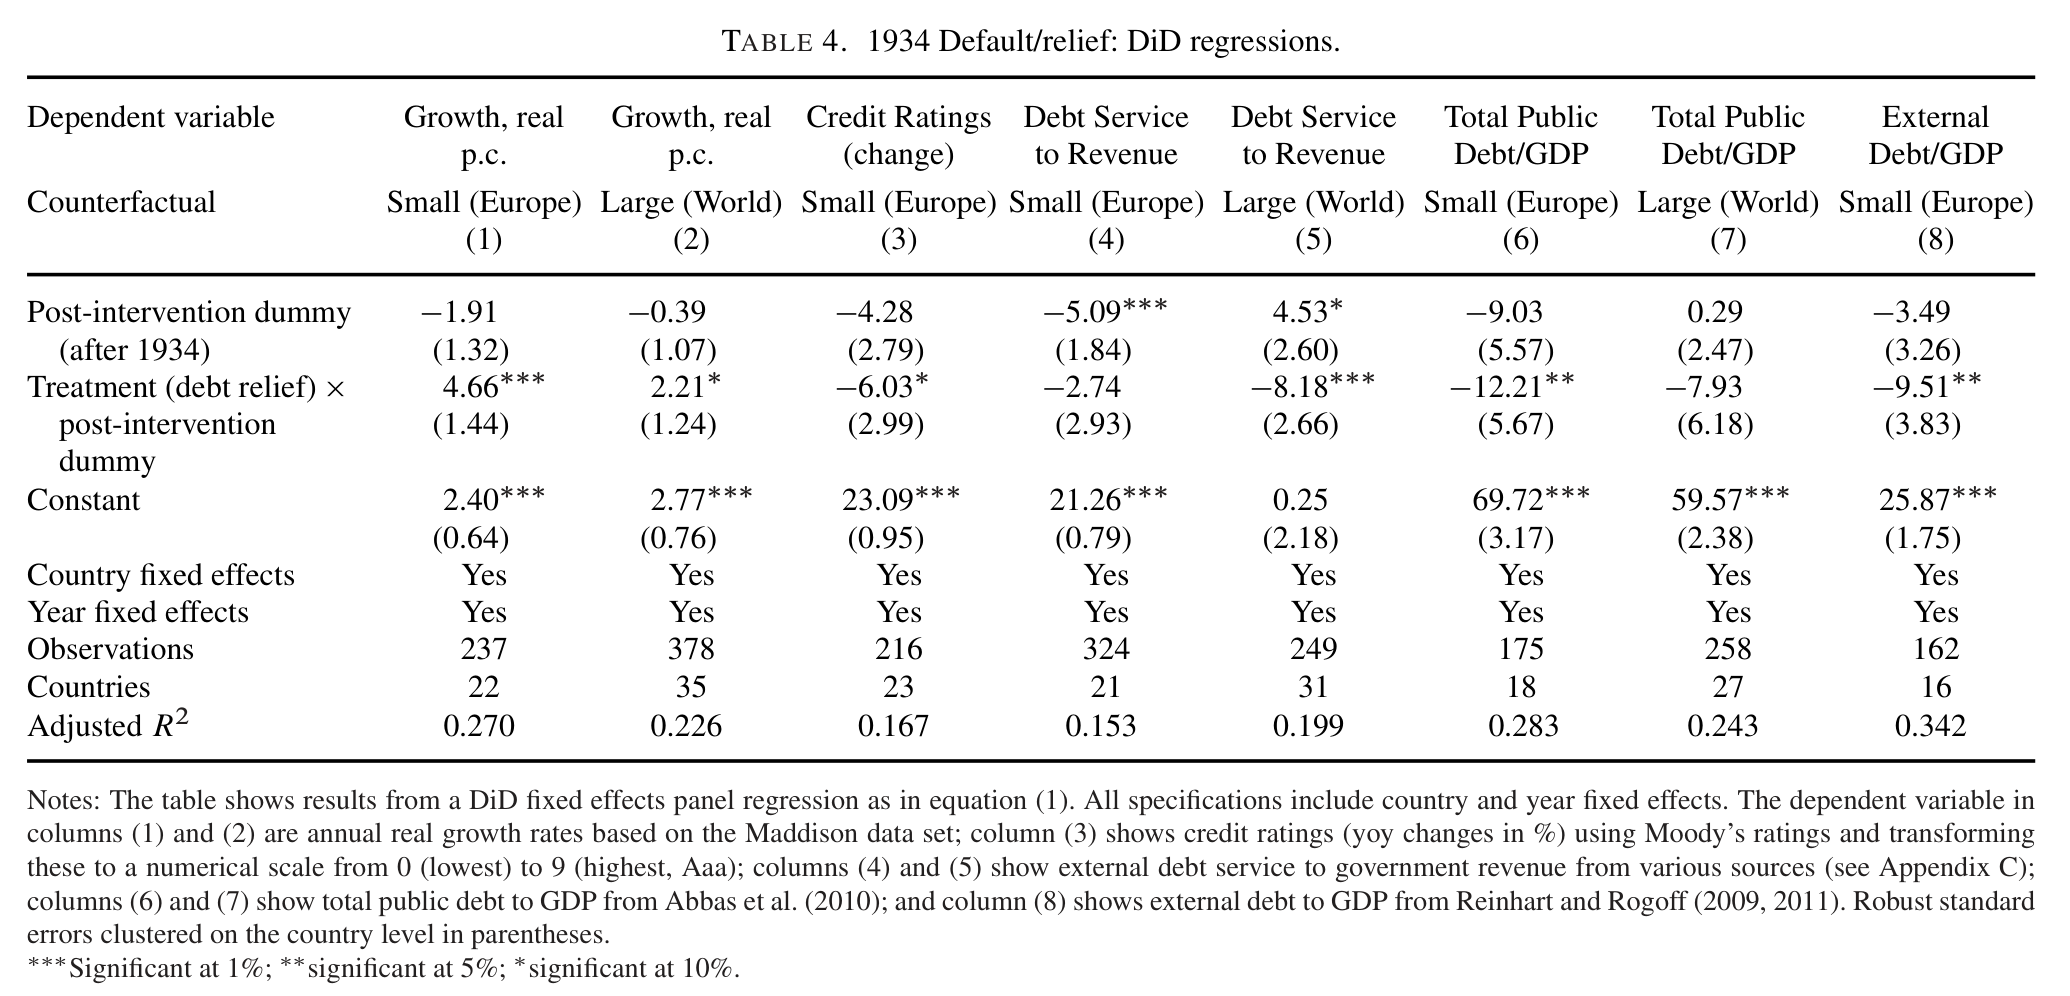
\includegraphics[width=0.95\linewidth]{figures/tab4.png}
      \captionof{figure}{\tiny 1934 Debt Relief Results}
      \label{fig:tab4}
  \end{figure}  
\end{frame}

\begin{frame}{Table 4 Replication: Data Inconsistencies Found}
  \frametitle{Major Discrepancies in Table 4 Results}
  \begin{itemize}
    \item \textbf{Column Order Issue}:
    \begin{itemize}
        \item Original Table 3 columns (3), (4), (5) appear to be in wrong order
        \item Correct data order should be: (5), (3), (4)
        \item This affects interpretation of debt service result
    \end{itemize}
  \end{itemize}
\end{frame}

\begin{frame}{War Period: Results of DID}
  \frametitle{Results of DID: 1934 Debt Relief Robustness Check}
  \begin{table}[ht!]\centering
      \renewcommand{\arraystretch}{1.1}
      \footnotesize
      \begin{tabular}{@{}p{2.2cm}ccccc@{}}
    \toprule
    \textbf{Specification} & \textbf{Treatment Effect} & \textbf{Std. Error} & \textbf{Observations} & \textbf{Adjusted R²} \\
    \midrule
    Baseline & $4.658^{***}$ & $(1.437)$ & 237 & 0.270 \\
    No Year FE & $4.667^{***}$ & $(1.392)$ & 237 & 0.135 \\
    3-Year Window & $4.002^{*}$ & $(2.013)$ & 132 & 0.186 \\
    4-Year Window & $3.952^{**}$ & $(1.845)$ & 175 & 0.272 \\
    6-Year Window & $4.658^{***}$ & $(1.437)$ & 237 & 0.270 \\
    Placebo 1933 & --- & --- & 218 & --- \\
    Excl. Treat Year & $4.625^{***}$ & $(1.533)$ & 215 & 0.265 \\
    With Inflation & $4.405^{**}$ & $(1.873)$ & 170 & 0.275 \\
    With Crises & $4.437^{**}$ & $(1.556)$ & 217 & 0.295 \\
    With Wars & $5.448^{***}$ & $(1.619)$ & 215 & 0.249 \\
    \bottomrule
    \end{tabular}
    % \begin{minipage}{\textwidth}
    % \footnotesize
    % \textbf{Notes:} This table presents robustness checks for the main result on the effect of the 1934 summer defaults on real per capita GDP growth. The baseline specification includes country and year fixed effects with standard errors clustered at the country level. Row (1) replicates the main result from Table 4. Rows (2)-(19) show results under various alternative specifications and sample restrictions. Treatment effect measures the impact of war debt default on GDP growth in the post-1934 period. The placebo test (row 6) uses 1933 as the false treatment year and shows no significant effect. Standard errors in parentheses. Significance levels: $^*$ p$<$0.10, $^{**}$ p$<$0.05, $^{***}$ p$<$0.01
    % \end{minipage}
    \end{table}
\end{frame}

\begin{frame}{War Period: Results of DID}
  \frametitle{Results of DID: 1934 Debt Relief Robustness Check}
  \begin{table}[ht!]\centering
      \renewcommand{\arraystretch}{1.1}
      \footnotesize
      \begin{tabular}{@{}p{2.2cm}cccc@{}}
    \toprule
    \textbf{Specification} & \textbf{Treatment Effect} & \textbf{Std. Error} & \textbf{Observations} & \textbf{Adjusted R²} \\
    \midrule
    With Politics & $3.933^{**}$ & $(1.684)$ & 215 & 0.281 \\
    No East Europe & $3.921^{**}$ & $(1.607)$ & 187 & 0.271 \\
    Europe Only & $4.553^{***}$ & $(1.583)$ & 215 & 0.245 \\
    No Germany & $4.440^{***}$ & $(1.487)$ & 226 & 0.261 \\
    No Aus/NZ & $4.553^{***}$ & $(1.583)$ & 215 & 0.246 \\
    No Large Relief & $5.192^{***}$ & $(1.639)$ & 204 & 0.261 \\
    No Small Relief & $4.203^{**}$ & $(1.543)$ & 204 & 0.281 \\
    No Best GDP & $3.577^{**}$ & $(1.473)$ & 204 & 0.244 \\
    No Worst GDP & $5.872^{***}$ & $(1.412)$ & 204 & 0.199 \\
    \bottomrule
    \end{tabular}
    \begin{minipage}{\textwidth}
    \footnotesize
    \textbf{Notes:} This table presents robustness checks for the main result on the effect of the 1934 summer defaults on real per capita GDP growth. The baseline specification includes country and year fixed effects with standard errors clustered at the country level. Row (1) replicates the main result from Table 4. Rows (2)-(19) show results under various alternative specifications and sample restrictions. Treatment effect measures the impact of war debt default on GDP growth in the post-1934 period. The placebo test (row 6) uses 1933 as the false treatment year and shows no significant effect. Standard errors in parentheses. Significance levels: $^*$ p$<$0.10, $^{**}$ p$<$0.05, $^{***}$ p$<$0.01
    \end{minipage}
    \end{table}
\end{frame}

\begin{frame}{War Period: Results of DID}
  \frametitle{Results of DID: 1934 Debt Relief}
  \textbf{Key findings from Table 4 (DID estimates):}
  \begin{itemize}
    \item \textbf{Real per capita growth}:
    \begin{itemize}
        \item \textcolor{green!70!black}{+4.7\% higher} for treated countries post-1934 (highly significant, vs. European non-defaulters).
        \item Remains large and significant across various counterfactuals (sometimes at 10\% level).
    \end{itemize}
    \item \textbf{Debt levels}:
    \begin{itemize}
        \item \textcolor{green!70!black}{Decrease significantly} (vs. European non-defaulters).
        \item Turns insignificant with "World" counterfactual.
    \end{itemize}
    \item \textbf{Debt servicing}:
    \begin{itemize}
        \item \textcolor{green!70!black}{Highly significant and large} (improvement) (vs. European non-defaulters).
        \item Becomes insignificant with ``World'' counterfactual.
    \end{itemize}
    \item \textbf{Ratings}:
    \begin{itemize}
        \item \textcolor{red}{Significant negative coefficient}.
    \end{itemize}
  \end{itemize}
  % \textit{Note: Results sensitive to choice of counterfactual.}
  % User can \input{mainmatter/Table4_DID.tex} here if formatted for Beamer
\end{frame}

\subsection{Emerging Markets}
\begin{frame}{Emerging Markets: Parallel Trend Test}
  \frametitle{Parallel Trend Test (Self-Conducted for EME)}
  Authors didn't construct PT tests for Baker and Brady initiatives either, only descriptive analysis.
  \begin{itemize}
    \item \textbf{Key Findings}:
    \begin{itemize}
        \item Most variables passed the parallel trend assumption.
        \item \alert{Interpret with caution for Baker Policy}:
        \begin{itemize}
            \item Credit rating results.
            \item Debt/GDP ratio results.
        \end{itemize}
    \end{itemize}
  \end{itemize}
  % \textit{(Again, select representative PT figures for EME from the report's 10 PT figures for EMEs.)}
  \begin{columns}
    \begin{column}{0.5\textwidth}
      \centering 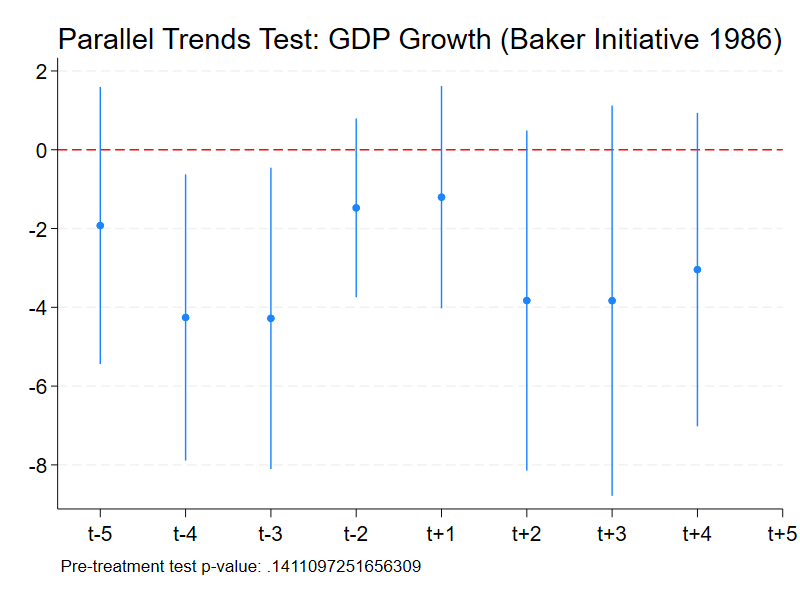
\includegraphics[width=0.8\linewidth]{figures/PT_Baker_GDP.png} 
      % \captionof{figure}{\tiny PT: Baker GDP}
    \end{column}
    \begin{column}{0.5\textwidth}
      \centering 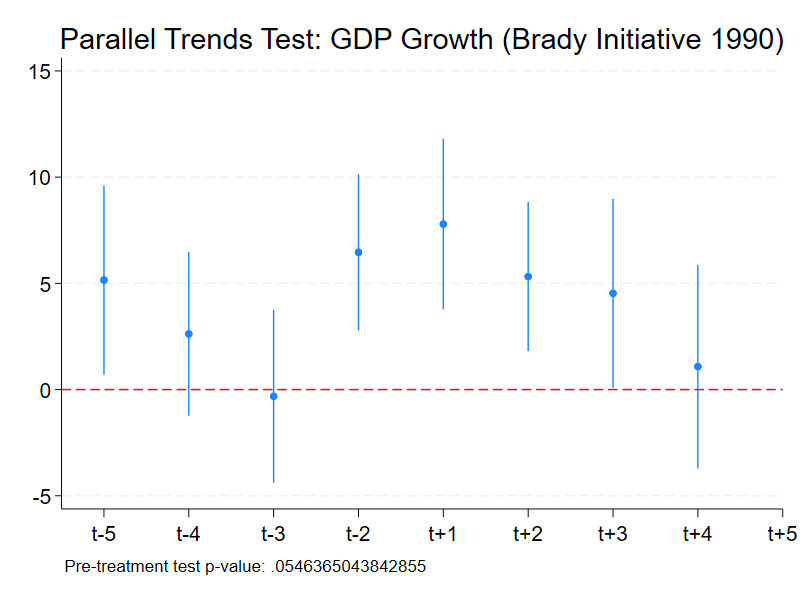
\includegraphics[width=0.8\linewidth]{figures/PT_Brady_GDP.png} 
      % \captionof{figure}{\tiny PT: Brady GDP}
    \end{column}
  \end{columns}
\end{frame}

\begin{frame}{EME: Parallel Trend Test (Cont'd)}
  \frametitle{Parallel Trend Test (Cont'd)}
  \begin{columns}[T] % T for top alignment
    \begin{column}{0.45\textwidth}
      \centering
      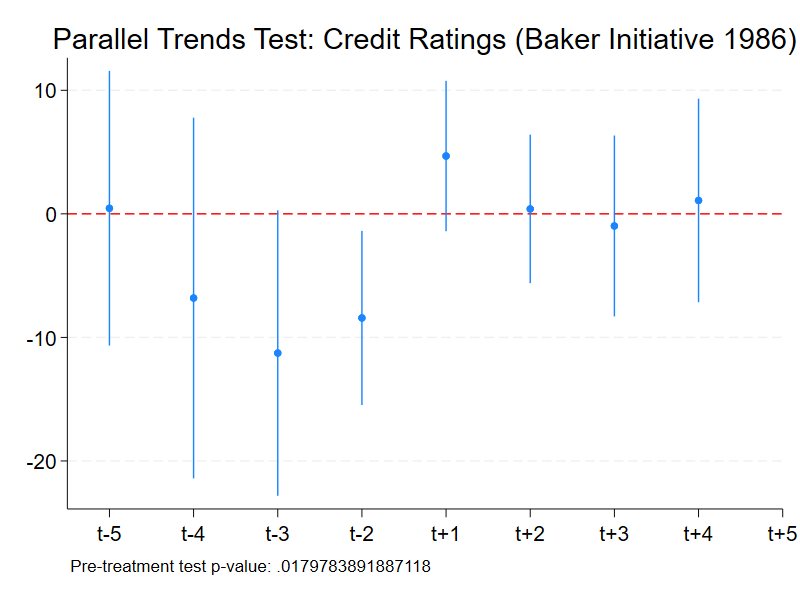
\includegraphics[width=0.9\linewidth]{figures/PT_Baker_Ratings.png}
      % \captionof{figure}{\tiny PT: Baker Rating}
      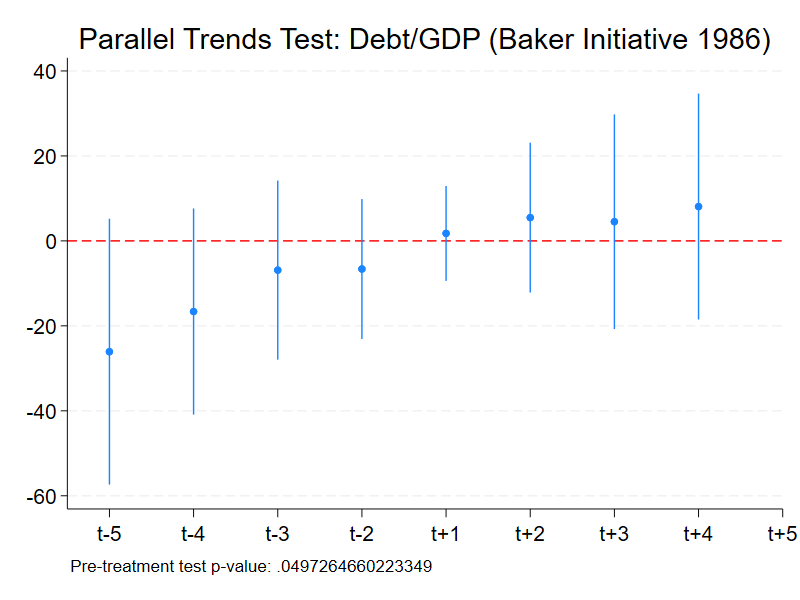
\includegraphics[width=0.9\linewidth]{figures/PT_Baker_Debt.png}
    \end{column}
    \begin{column}{0.45\textwidth}
      \centering
      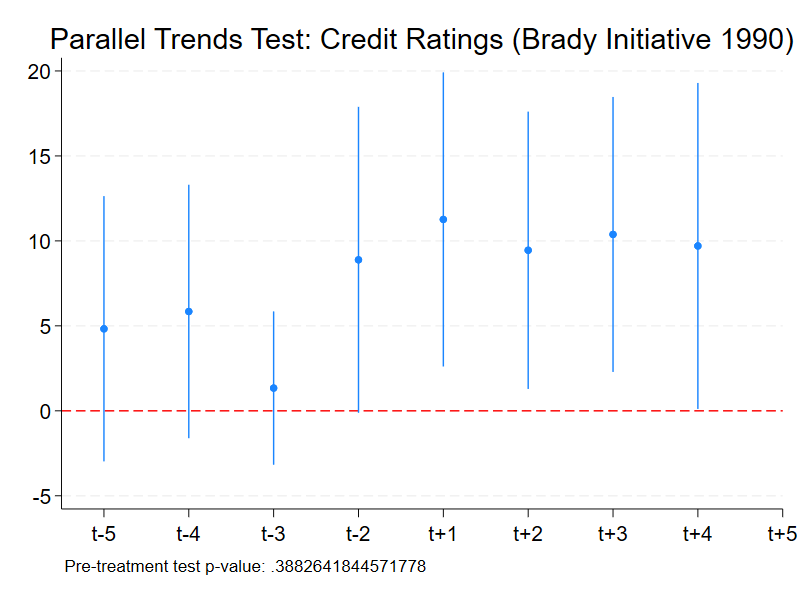
\includegraphics[width=0.9\linewidth]{figures/PT_Brady_Ratings.png}
      % \captionof{figure}{\tiny PT: Brady Rating}
      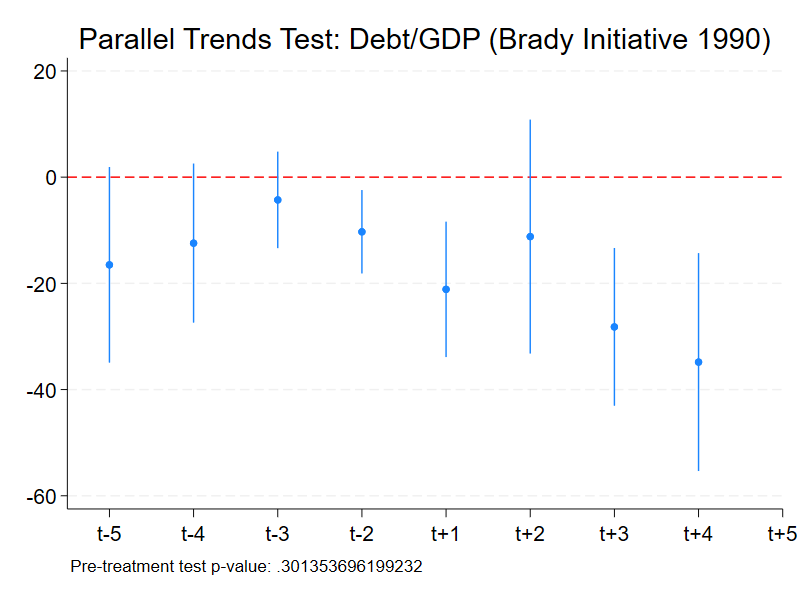
\includegraphics[width=0.9\linewidth]{figures/PT_Brady_Debt.png}
    \end{column}
  \end{columns}
\end{frame}

\begin{frame}{EME: Parallel Trend Test (Cont'd)}
  \frametitle{Parallel Trend Test (Cont'd)}
  \begin{columns}[T] % T for top alignment
    \begin{column}{0.45\textwidth}
      \centering
      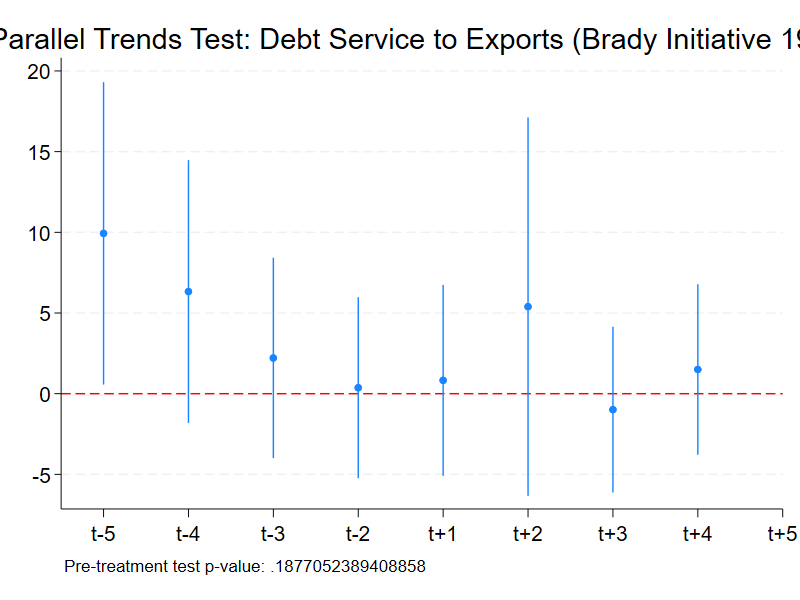
\includegraphics[width=0.9\linewidth]{figures/PT_Brady_DebtServ.png}
      % \captionof{figure}{\tiny PT: Baker Rating}
      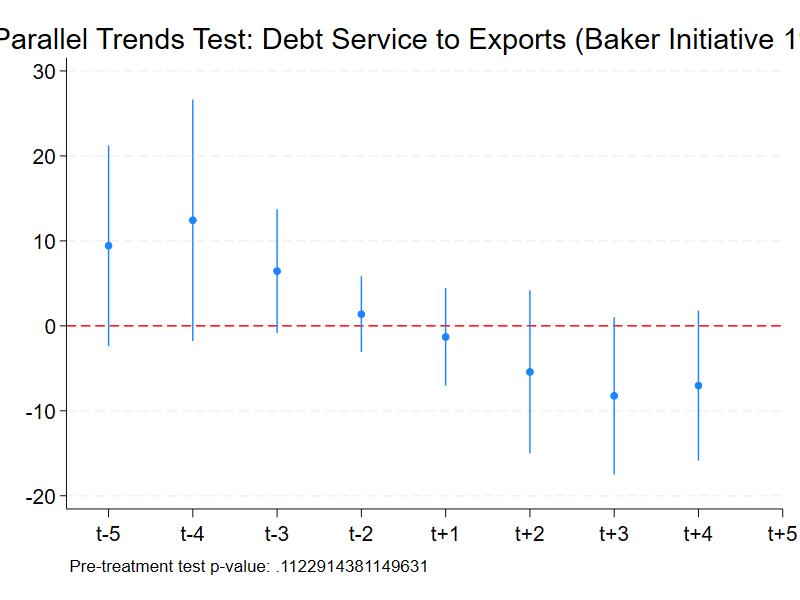
\includegraphics[width=0.9\linewidth]{figures/PT_Baker_DebtServ.png}
    \end{column}
    \begin{column}{0.45\textwidth}
      \centering
      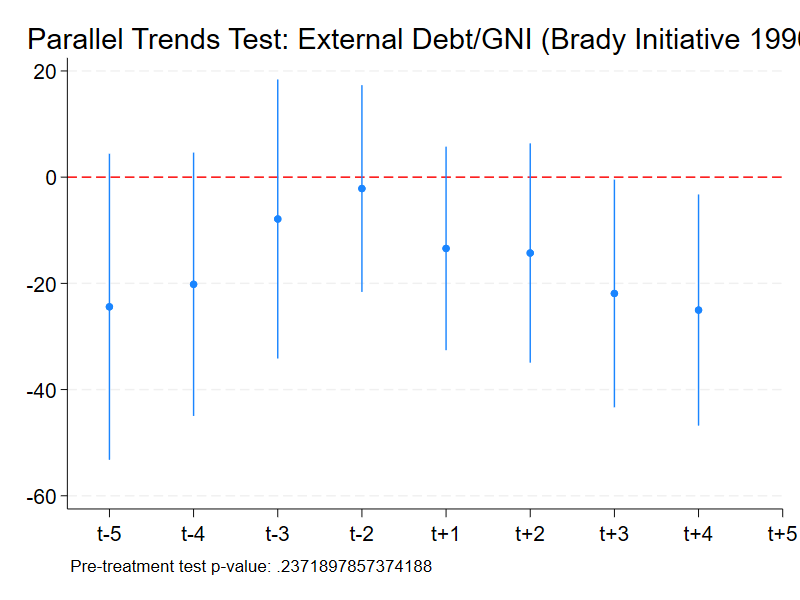
\includegraphics[width=0.9\linewidth]{figures/PT_Brady_ExtDebt.png}
      % \captionof{figure}{\tiny PT: Brady Rating}
      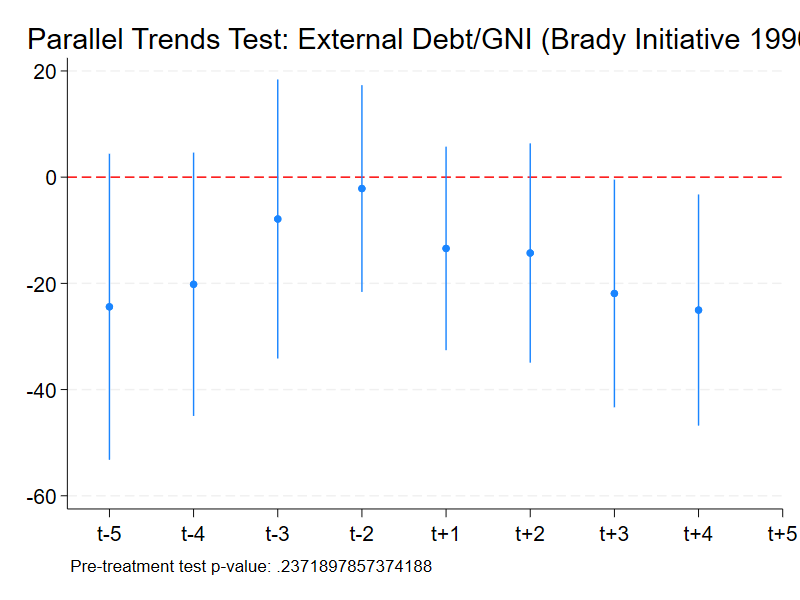
\includegraphics[width=0.9\linewidth]{figures/PT_Brady_ExtDebt.png}
    \end{column}
  \end{columns}
\end{frame}

\begin{frame}{Emerging Markets: Baker Episode}
  \frametitle{Brady Episode DID Results}
    \begin{table}[ht!]\centering
      \renewcommand{\arraystretch}{1.1}
      \footnotesize
      \begin{tabular}{@{}p{2.2cm}ccccc@{}}
      \toprule
                  &(1)&(2)&(3)&(4)&(5)\\
                  &\parbox{1.2cm}{\centering\footnotesize Growth, real p.c.}&\parbox{1.2cm}{\centering\footnotesize Credit Ratings (change)}&\parbox{1.2cm}{\centering\footnotesize Debt Service to Exports}&\parbox{1.2cm}{\centering\footnotesize Total Public Debt/GDP}&\parbox{1.2cm}{\centering\footnotesize External Debt/GNI}\\
      \midrule
      \parbox{4cm}{\raggedright Post-1986 dummy}&  $-1.976$  &  $-5.968^{**}$  &  $-5.758$  &  $-17.214^{**}$  &  $-8.881$  \\
            &  $(1.292)$  &  $(2.328)$ & $(3.426)$   &  $(7.106)$   &  $(6.251)$  \\
      \parbox{4cm}{\raggedright Baker Treatment $\times$ Post-1986}&  $-1.918$&  $6.305^{*}$  &  $-9.049^{*}$&  $22.988^{**}$  &  $17.432$   \\
                  &  $(1.329)$   &  $(3.121)$   &  $(4.720)$   &  $(9.360)$   &  $(10.802)$   \\
      \midrule
      Observations&       $275$   &       $279$   &       $189$   &       $226$   &       $199$   \\
      % R-squared   &       $0.111$   &       $0.200$   &       $0.154$   &       $0.238$   &       $0.189$   \\
      Adjusted R² &       $0.077$   &       $0.170$   &       $0.106$   &       $0.203$   &       $0.145$   \\
      \bottomrule
      \end{tabular}
  \end{table}
\end{frame}

\begin{frame}{Emerging Markets: Baker Episode}
  \frametitle{Baker Episode DID Results}
    \begin{columns}[T] % T for top alignment
    \begin{column}{0.45\textwidth}
      \centering
      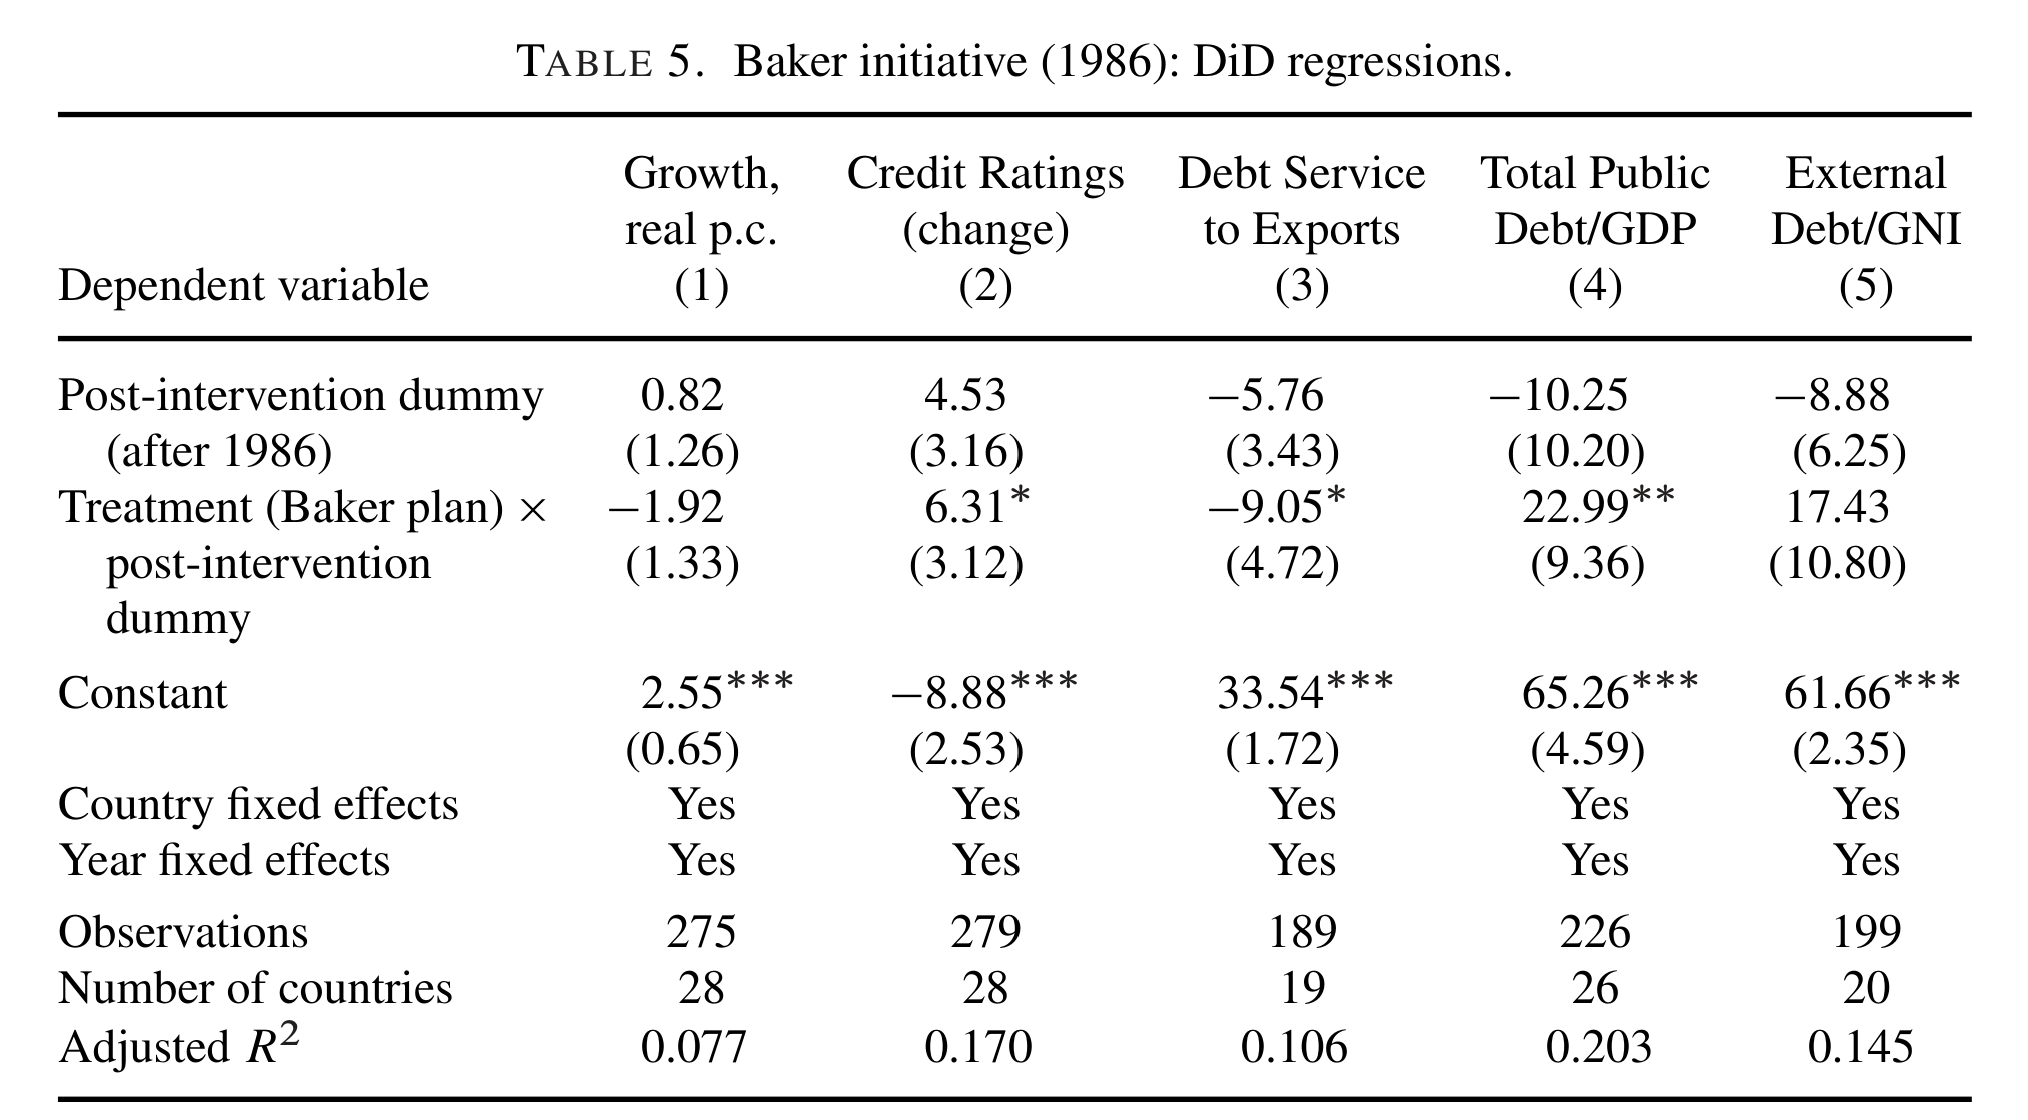
\includegraphics[width=0.9\linewidth]{figures/tab5.png}
    \end{column}
    \begin{column}{0.45\textwidth}
      \centering
      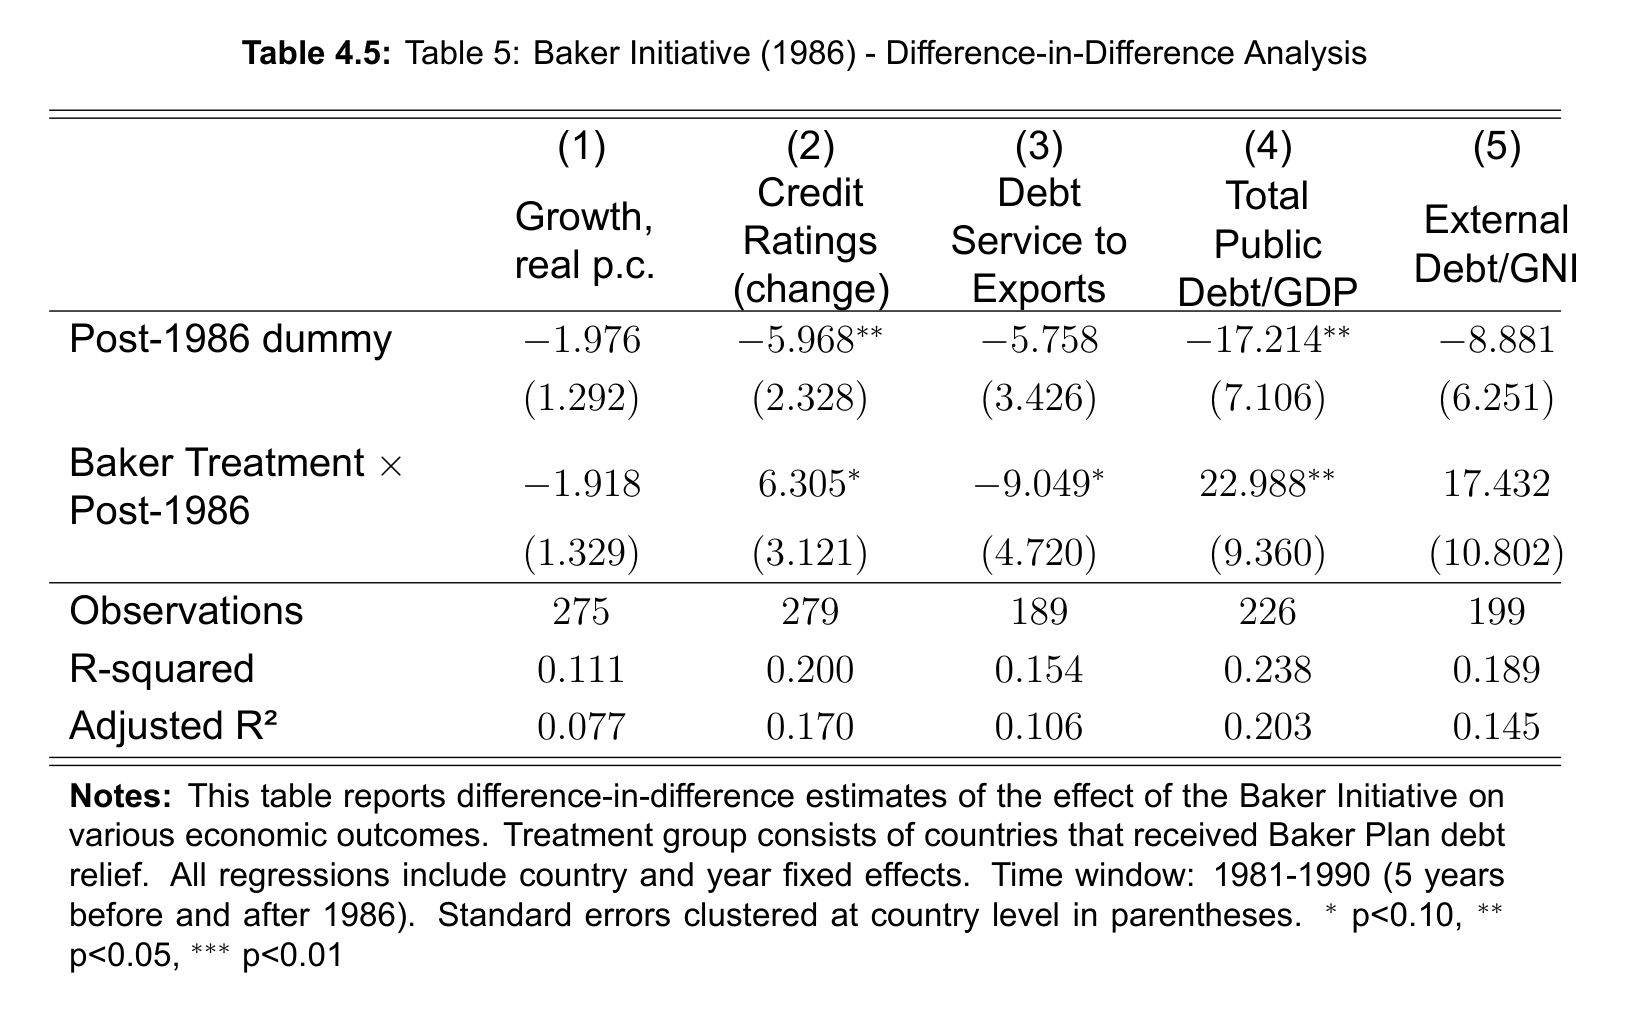
\includegraphics[width=0.9\linewidth]{figures/tab5_rep.png}
    \end{column}
  \end{columns}
  \textbf{Key findings from Table 5:}
  \begin{itemize}
    \item \textbf{Output growth}: Negative and insignificant treatment coefficient.
    \item \textbf{Debt/GDP}: Continues to grow post-treatment.
    \item \textbf{Credit ratings}: \textcolor{green!70!black}{Increase significantly more} for Baker countries than counterfactual (window includes early Brady years).
    \item \textbf{Debt servicing}: Treatment coefficient negative and marginally significant (\textcolor{green!70!black}{cash flow relief}).
  \end{itemize}
  % User can \begin{table}[ht!]\centering
\def\sym#1{\ifmmode^{#1}\else\(^{#1}\)\fi}
\caption{Table 5: Baker Initiative (1986) - Difference-in-Difference Analysis}
\renewcommand{\arraystretch}{1.2} % 增加行距
\begin{tabular*}{\textwidth}{@{\hskip\tabcolsep\extracolsep\fill}p{4cm}*{5}{>{\centering\arraybackslash}p{2cm}}}
\hline\hline
            &(1)&(2)&(3)&(4)&(5)\\
            &\parbox{2cm}{\centering Growth, real p.c.}&\parbox{2cm}{\centering Credit Ratings (change)}&\parbox{2cm}{\centering Debt Service to Exports}&\parbox{2cm}{\centering Total Public Debt/GDP}&\parbox{2cm}{\centering External Debt/GNI}\\
\hline
\parbox{4cm}{\raggedright Post-1986 dummy}&  $-1.976$  &  $-5.968^{**}$  &  $-5.758$  &  $-17.214^{**}$  &  $-8.881$  \\
            &  $(1.292)$  &  $(2.328)$ & $(3.426)$   &  $(7.106)$   &  $(6.251)$  \\
[0.5em]
\parbox{4cm}{\raggedright Baker Treatment $\times$ Post-1986}&  $-1.918$&  $6.305^{*}$  &  $-9.049^{*}$&  $22.988^{**}$  &  $17.432$   \\
            &  $(1.329)$   &  $(3.121)$   &  $(4.720)$   &  $(9.360)$   &  $(10.802)$   \\
\hline
Observations&       $275$   &       $279$   &       $189$   &       $226$   &       $199$   \\
R-squared   &       $0.111$   &       $0.200$   &       $0.154$   &       $0.238$   &       $0.189$   \\
Adjusted R² &       $0.077$   &       $0.170$   &       $0.106$   &       $0.203$   &       $0.145$   \\
\hline\hline
\multicolumn{6}{p{0.95\textwidth}}{\footnotesize \textbf{Notes:} This table reports difference-in-difference estimates of the effect of the Baker Initiative on various economic outcomes. Treatment group consists of countries that received Baker Plan debt relief. All regressions include country and year fixed effects. Time window: 1981-1990 (5 years before and after 1986). Standard errors clustered at country level in parentheses. $^*$ p<0.10, $^{**}$ p<0.05, $^{***}$ p<0.01}\\
\end{tabular*}
\end{table}
 here
\end{frame}

\begin{frame}{Emerging Markets: Brady Episode}
  \frametitle{Brady Episode DID Results}
  %   \begin{columns}[T] % T for top alignment
  %   \begin{column}{0.45\textwidth}
  %     \centering
  %     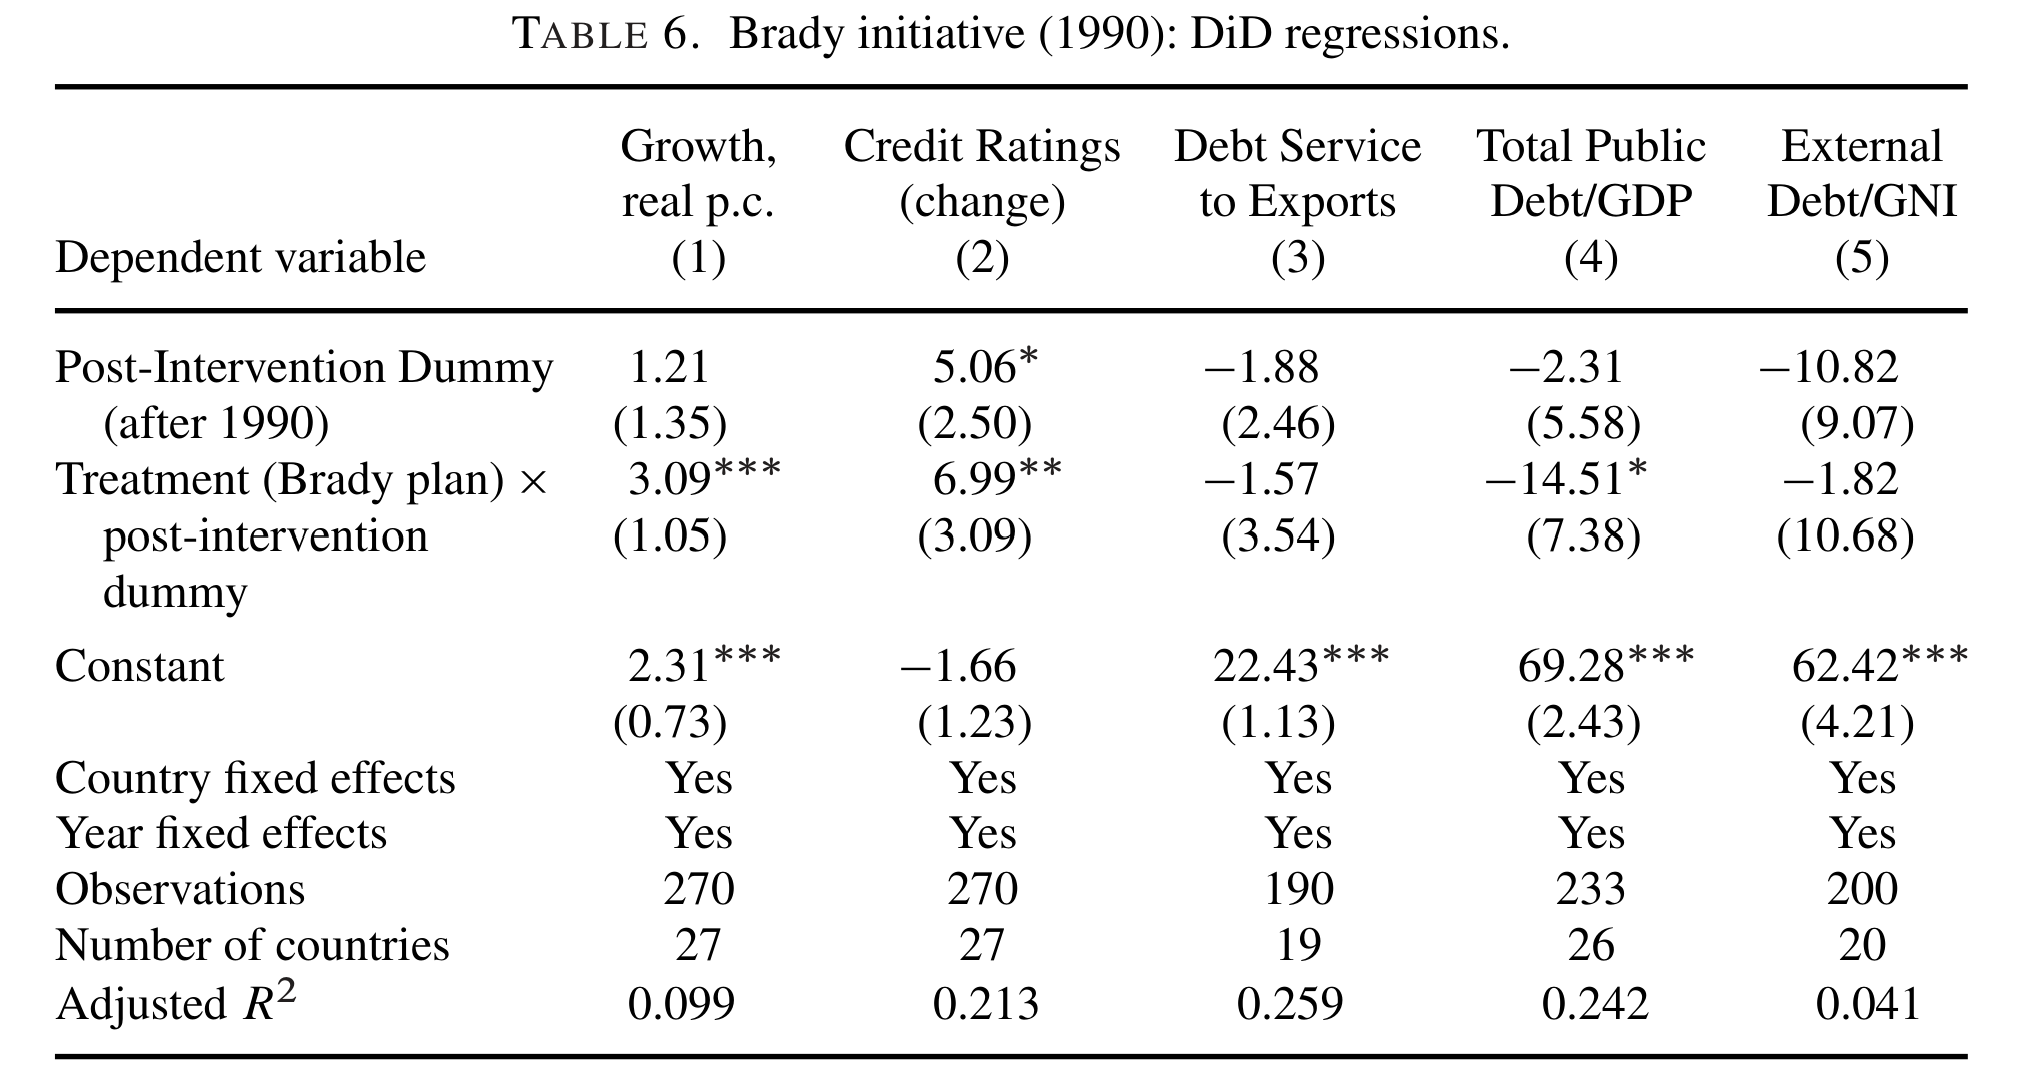
\includegraphics[width=0.9\linewidth]{figures/tab6.png}
  %   \end{column}
  %   \begin{column}{0.45\textwidth}
  %     \centering
  %     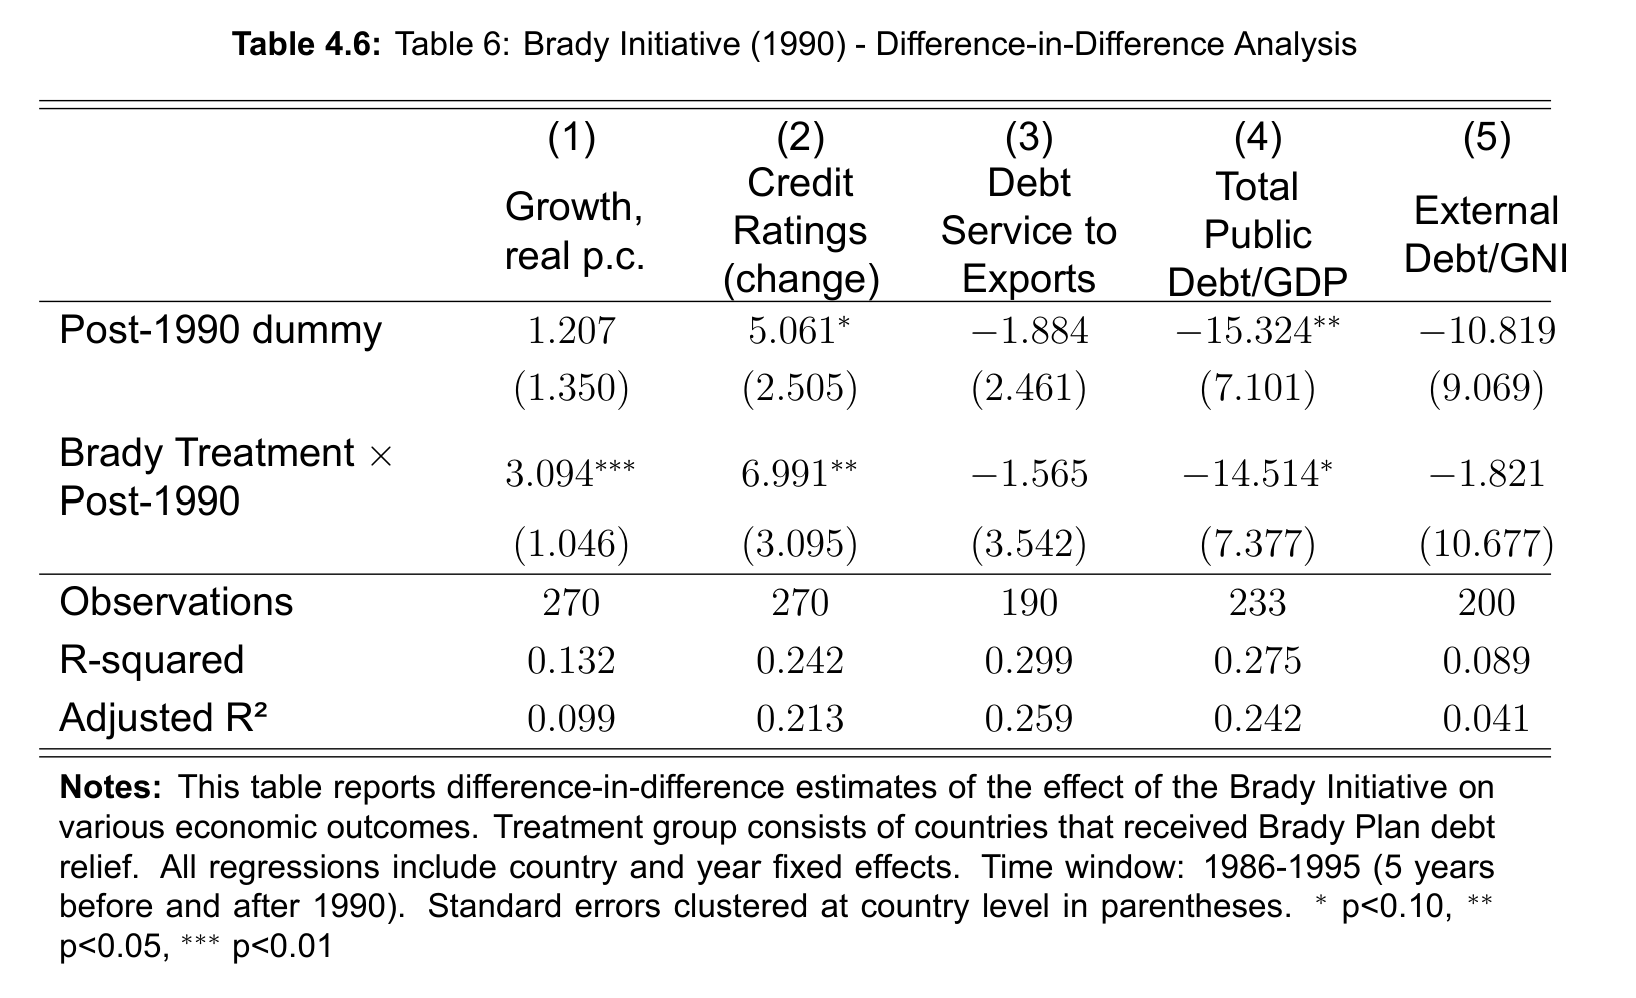
\includegraphics[width=0.9\linewidth]{figures/tab6_rep.png}
  %   \end{column}
  % \end{columns}
  \begin{table}[ht!]\centering
    \renewcommand{\arraystretch}{1.1}
    \footnotesize
    \begin{tabular}{@{}p{2.2cm}ccccc@{}}
    \toprule
                &(1)&(2)&(3)&(4)&(5)\\
                &\parbox{1.2cm}{\centering\footnotesize Growth, real p.c.}&\parbox{1.2cm}{\centering\footnotesize Credit Ratings (change)}&\parbox{1.2cm}{\centering\footnotesize Debt Service to Exports}&\parbox{1.2cm}{\centering\footnotesize Total Public Debt/GDP}&\parbox{1.2cm}{\centering\footnotesize External Debt/GNI}\\
    \midrule
    \parbox{2.2cm}{\raggedright\footnotesize Post-1990 dummy}&  $1.207$  &  $5.061^*$  &  $-1.884$  &  $-15.324^{**}$  &  $-10.819$  \\
                &  $(1.350)$  &  $(2.505)$ & $(2.461)$   &  $(7.101)$   &  $(9.069)$  \\
    [0.3em]
    \parbox{2.2cm}{\raggedright\footnotesize Brady Treatment $\times$ Post-1990}&  $3.094^{***}$&  $6.991^{**}$  &  $-1.565$&  $-14.514^*$  &  $-1.821$   \\
                &  $(1.046)$   &  $(3.095)$   &  $(3.542)$   &  $(7.377)$   &  $(10.677)$   \\
    \midrule
    Observations&       $270$   &       $270$   &       $190$   &       $233$   &       $200$   \\
    % R-squared   &       $0.132$   &       $0.242$   &       $0.299$   &       $0.275$   &       $0.089$   \\
    Adjusted R² &       $0.099$   &       $0.213$   &       $0.259$   &       $0.242$   &       $0.041$   \\
    \bottomrule
    \end{tabular}
  \end{table}
\end{frame}

\begin{frame}{Emerging Markets: Brady Episode}
  \textbf{Key findings from Table 6 (compared to Baker):}
  \begin{itemize}
    \item \textbf{Real per capita GDP growth}:
    \begin{itemize}
        \item Treatment coefficient turns \textcolor{green!70!black}{positive and highly significant}.
        \item Indicates \textcolor{green!70!black}{$\sim$3 \% higher growth} for Brady countries vs. counterfactual.
        \item Resembles 1934 episode.
    \end{itemize}
    \item \textbf{Credit ratings}: Large improvement relative to counterfactual 
    % (\textcolor{green!70!black}{$\sim$7 IIR index points}).
    \item \textbf{Government debt levels}: Drop significantly more (\textcolor{green!70!black}{by 15 \%}).
    \item \textbf{Debt servicing \& Total external debt/GDP}: Surprisingly, no significant effect.
    \begin{itemize}
        \item Possible reason: Actual Brady restructurings occurred with a lag in many countries.
    \end{itemize}
  \end{itemize}
  % User can \begin{table}[ht!]\centering
\def\sym#1{\ifmmode^{#1}\else\(^{#1}\)\fi}
\caption{Table 6: Brady Initiative (1990) - Difference-in-Difference Analysis}
\renewcommand{\arraystretch}{1.2} % 增加行距
\begin{tabular*}{\textwidth}{@{\hskip\tabcolsep\extracolsep\fill}p{4cm}*{5}{>{\centering\arraybackslash}p{2cm}}}
\hline\hline
            &(1)&(2)&(3)&(4)&(5)\\
            &\parbox{2cm}{\centering Growth, real p.c.}&\parbox{2cm}{\centering Credit Ratings (change)}&\parbox{2cm}{\centering Debt Service to Exports}&\parbox{2cm}{\centering Total Public Debt/GDP}&\parbox{2cm}{\centering External Debt/GNI}\\
\hline
\parbox{4cm}{\raggedright Post-1990 dummy}&  $1.207$  &  $5.061^*$  &  $-1.884$  &  $-15.324^{**}$  &  $-10.819$  \\
            &  $(1.350)$  &  $(2.505)$ & $(2.461)$   &  $(7.101)$   &  $(9.069)$  \\
[0.5em]
\parbox{4cm}{\raggedright Brady Treatment $\times$ Post-1990}&  $3.094^{***}$&  $6.991^{**}$  &  $-1.565$&  $-14.514^*$  &  $-1.821$   \\
            &  $(1.046)$   &  $(3.095)$   &  $(3.542)$   &  $(7.377)$   &  $(10.677)$   \\
\hline
Observations&       $270$   &       $270$   &       $190$   &       $233$   &       $200$   \\
R-squared   &       $0.132$   &       $0.242$   &       $0.299$   &       $0.275$   &       $0.089$   \\
Adjusted R² &       $0.099$   &       $0.213$   &       $0.259$   &       $0.242$   &       $0.041$   \\
\hline\hline
\multicolumn{6}{p{0.95\textwidth}}{\footnotesize \textbf{Notes:} This table reports difference-in-difference estimates of the effect of the Brady Initiative on various economic outcomes. Treatment group consists of countries that received Brady Plan debt relief. All regressions include country and year fixed effects. Time window: 1986-1995 (5 years before and after 1990). Standard errors clustered at country level in parentheses. $^*$ p<0.10, $^{**}$ p<0.05, $^{***}$ p<0.01}\\
\end{tabular*}
\end{table}
 here
\end{frame}


\subsection{Staggered DID Analysis (Brady Plan)}
\begin{frame}{Staggered DID Analysis: Brady Plan Context}
  \begin{itemize}
    \item \textbf{Motivation}: Brady Plan implemented in a staggered fashion (from Arslanalp and Henry (2005)).
    \item \textbf{Methodology}: Callaway-Sant'Anna (2021) staggered DID (CSDID) estimator.
    \begin{itemize}
        \item Allows for heterogeneous and dynamic treatment effects.
    \end{itemize}
  \end{itemize}
  % \textit{The report shows 5 CSDID figures. Below are examples for Growth and Debt.}
  \begin{columns}
    \begin{column}{0.5\textwidth}
      \centering
      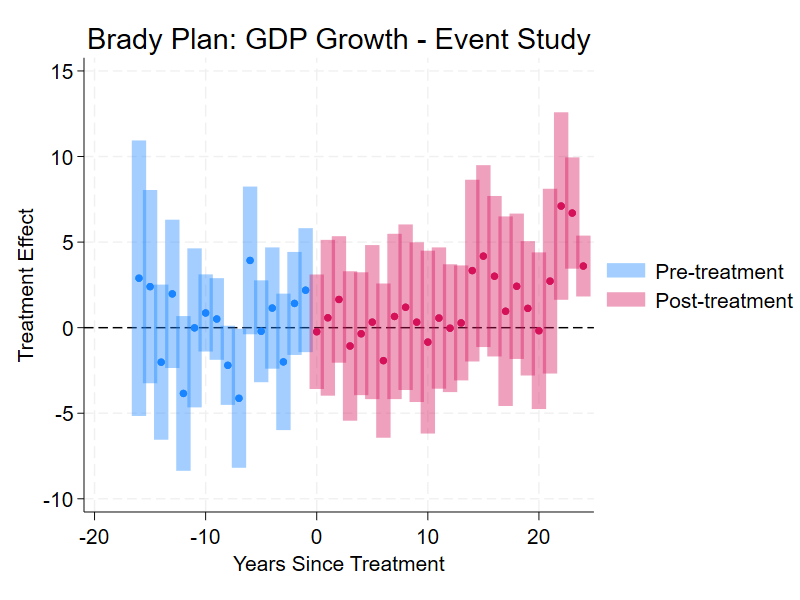
\includegraphics[width=0.9\linewidth]{figures/CS_Brady_Growth_EventStudy.png}
    \end{column}
    \begin{column}{0.5\textwidth}
      \centering
      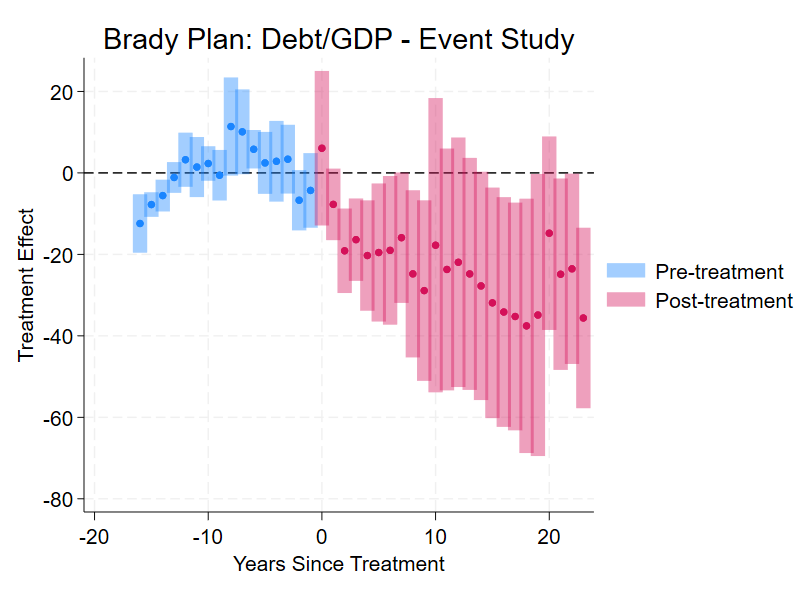
\includegraphics[width=0.9\linewidth]{figures/CS_Brady_Debt_EventStudy.png}
    \end{column}
  \end{columns}
\end{frame}

\begin{frame}{Staggered DID Analysis: Brady Plan Context}
  \begin{columns}
    \begin{column}{0.45\textwidth}
      \centering
      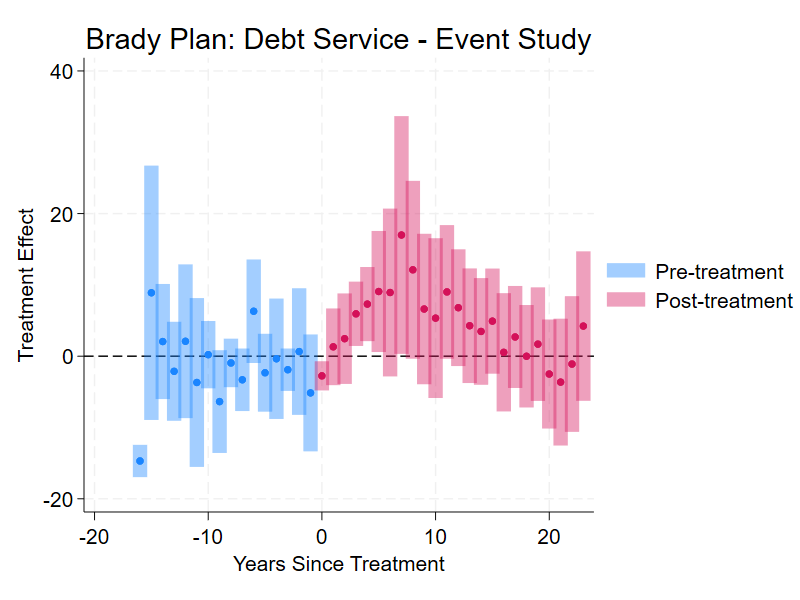
\includegraphics[width=0.9\linewidth]{figures/CS_Brady_DebtService_EventStudy.png}
      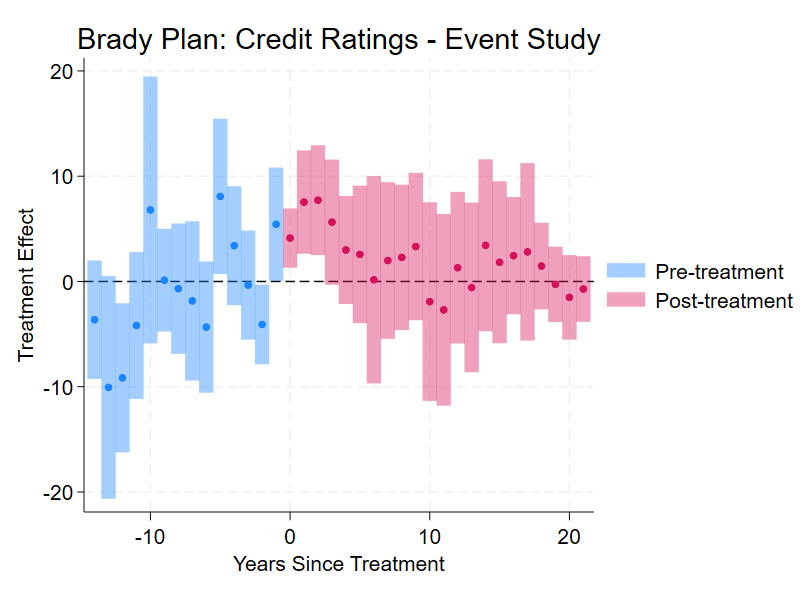
\includegraphics[width=0.9\linewidth]{figures/CS_Brady_Ratings_EventStudy.png}
    \end{column}
    \begin{column}{0.45\textwidth}
      \centering
      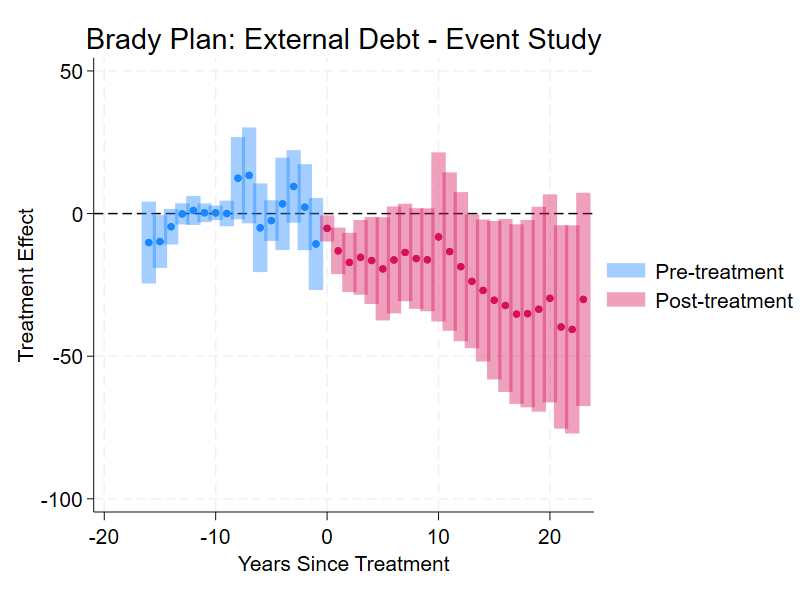
\includegraphics[width=0.9\linewidth]{figures/CS_Brady_ExtDebt_EventStudy.png}
    \end{column}
  \end{columns}
\end{frame}

\begin{frame}{Staggered DID: Results}
  \frametitle{CSDID Results for Brady Plan}
  \begin{table}[ht!]\centering
  \renewcommand{\arraystretch}{1.1}
  \footnotesize
  \begin{tabular}{@{}p{2.2cm}ccccc@{}}
  \toprule
              &(1)&(2)&(3)&(4)&(5)\\
              &\parbox{1.2cm}{\centering\footnotesize Growth, real p.c.}&\parbox{1.2cm}{\centering\footnotesize Credit Ratings (change)}&\parbox{1.2cm}{\centering\footnotesize Debt Service to Exports}&\parbox{1.2cm}{\centering\footnotesize Total Public Debt/GDP}&\parbox{1.2cm}{\centering\footnotesize External Debt/GNI}\\
  \midrule
  \parbox{2.2cm}{\raggedright\footnotesize Average Treatment Effect on Treated (ATT)}&  $1.005$  &  $2.331$  &  $5.047$  &  $-22.587^{**}$  &  $-20.799^{**}$  \\
              &  $(1.923)$  &  $(2.494)$ & $(3.299)$   &  $(9.722)$   &  $(9.550)$  \\
  [0.3em]
  \midrule
  Treatment Countries&       $16$   &       $16$   &       $16$   &       $16$   &       $16$   \\
  Control Countries   &       $24$   &       $24$   &       $24$   &       $24$   &       $24$   \\
  \bottomrule
  \end{tabular}
  \end{table}
  \vspace{0.3cm}
  \begin{footnotesize}
  \textbf{Notes:} Average treatment effects on the treated (ATT) from Callaway-Sant'Anna (2021) staggered DID estimator. Treatment timing: 1989-1995. Control group: emerging markets that never implemented Brady agreements. Standard errors clustered at country level. $^*$ p$<$0.10, $^{**}$ p$<$0.05, $^{***}$ p$<$0.01
  \end{footnotesize}
\end{frame}

\begin{frame}{Staggered DID Analysis: Results (Table Summary)}
  \frametitle{CSDID Results for Brady Plan (Summary)}
  \textbf{Key findings}
  \begin{itemize}
    \item \textbf{Real p.c. GDP growth}: $ATT = 1.005$ $(s.e. 1.923)$ $\rightarrow$ Small, insignificant.
    \item \textbf{Credit-rating upgrades}: $ATT = 2.331$ $(s.e. 2.494)$ $\rightarrow$ Imprecisely measured.
    \item \textbf{Debt-service to exports ratio}: $ATT = 5.047$ $(s.e. 3.299)$ $\rightarrow$ Rises, but insignificant (plausible due to front-loaded Brady bond coupons).
    \item \textbf{Public-debt burden (to GDP)}: $ATT = -22.587$ $(s.e. 9.722)$ $\rightarrow$ Statistically significant fall.
    \item \textbf{External indebtedness (to GNI)}: $ATT = -20.799$ $(s.e. 9.550)$ $\rightarrow$ Statistically significant fall.
  \end{itemize}
   \textit{Overall ATT from event study aggregation. Double stars ($^{**}$) in report text indicate significance.}
\end{frame}

\begin{frame}{Staggered DID Analysis: Implications \& Limitations}
  \textbf{Methodological Strengths:}
  \begin{itemize}
    \item CSDID avoids negative-weight bias of TWFE in staggered settings.
    \item Doubly robust inverse-probability weighting (DRIPW) enhances credibility.
  \end{itemize}
  \textbf{Economic Implications:}
  \begin{itemize}
    \item \textit{Debt relief first, growth later}: Significant debt reduction, but immediate growth dividends limited.
    \item \textit{Market sentiment lags policy action}: Ratings agencies reacted cautiously.
    \item \textit{Policy design}: Future restructurings should pair with complementary reforms.
  \end{itemize}
  \textbf{Limitations:}
  \begin{itemize}
    % \item Evaluation window (1989-1995) captures only initial 6 years post-exchange; growth effects might have longer lags.
    \item Macro-shocks in early 1990s (e.g., Tequila crisis) may attenuate observed effects despite DID controls.
  \end{itemize}
\end{frame}

\section{Conclusion}
\begin{frame}{Summary of Replication Findings}
  This presentation summarized a detailed replication effort covering:
  \begin{itemize}
    % \item \textbf{Historical Context}: The 1934 general default and its data sources.
    \item \textbf{Econometric Models}:
    \begin{itemize}
        \item Standard DID for analyzing debt relief events (1931, 1934, Baker, Brady).
        % \item Haircut calculation methodologies (WCR, Cumulative Haircut, DR to GDP).
        \item Extended discussion on Staggered DID for events like the Brady Plan.
    \end{itemize}
    \item \textbf{Empirical Replication}:
    \begin{itemize}
        \item Sample definitions and time windows for war period and EME analysis.
        \item Self-conducted Parallel Trend Tests for various episodes and samples.
        \item DID results:
            \begin{itemize}
                \item 1934: Positive growth effects, debt reduction (sensitive to counterfactual).
                \item Baker: Limited positive impact, some cash flow relief.
                \item Brady (standard DID): Positive growth, improved ratings, debt reduction.
            \end{itemize}
        \item Staggered DID for Brady: Significant debt reduction, but less clear immediate impact on growth or ratings in the short-term.
    \end{itemize}
  \end{itemize}
  % The replication highlights the nuances of debt relief effects and the importance of appropriate econometric techniques.
\end{frame}

\begin{frame}
  \centering
  \Huge Thank You! \par \bigskip
  % \Large Questions?
\end{frame}

\end{document}